% Chapter Template
\chapter{Gene circuit definition, exploration and parametrisation} \label{chapter2}
Up to now, Turing circuits that give rise to regular patterns, have only been engineered in chemical systems.
Using synthetic biology, we aimed to engineer Turing patterns in biological systems using gene circuits that exhibit reaction-diffusion (RD).
An RD synthetic gene circuit was built in~\cite{Tica2020}
using gene regulatory functions and quorum sensing components.
The reaction term comes from activation or inhibition by proteins binding to promoter or operator regions upstream of a gene
and regulating its expression.
The diffusion term describes the quorum-sensing molecules acting as morphogens and diffusing across the tissue,
as well as forming complexes with receptors to regulate gene expression.
Transitioning from a synthetic RD circuit to the generation of Turing patterns is not a trivial task due to the lack of parametric robustness of Turing systems.
To address this complex task, a model is needed which can help us understand the dynamic behaviour of the RD gene circuit and whether it can produce patterns.
Additionally, because of the lack of parametric robustness, it is important to learn how to tune parameters to increase the probability of obtaining patterns.

In this chapter, we present a model which describes this gene circuit.
Additionally, we explore the parameter space based on literature-informed ranges to understand what fraction of it leads to Turing and how to tune the circuit to obtain a higher probability of patterning.
Finally, to obtain a model which is more closely linked to our experimental system and yields more accurate predictions,
we parametrise it using liquid culture data.

Work in this chapter and the following Chapter~\ref{chapter3} has been published as a preprint in~\cite{Oliver2023}.
\section{Building model describing synthetic gene circuit}
In this section, I present a model which describes the synthetic gene circuit engineered in~\cite{Tica2020}.
The circuit can be seen in Fig.~\ref{fig:synthetic circuit_chapter2}, which was already presented in Chapter~\ref{introduction} but is repeated here to facilitate access to the reader.

\begin{figure}[H]
    \centering
    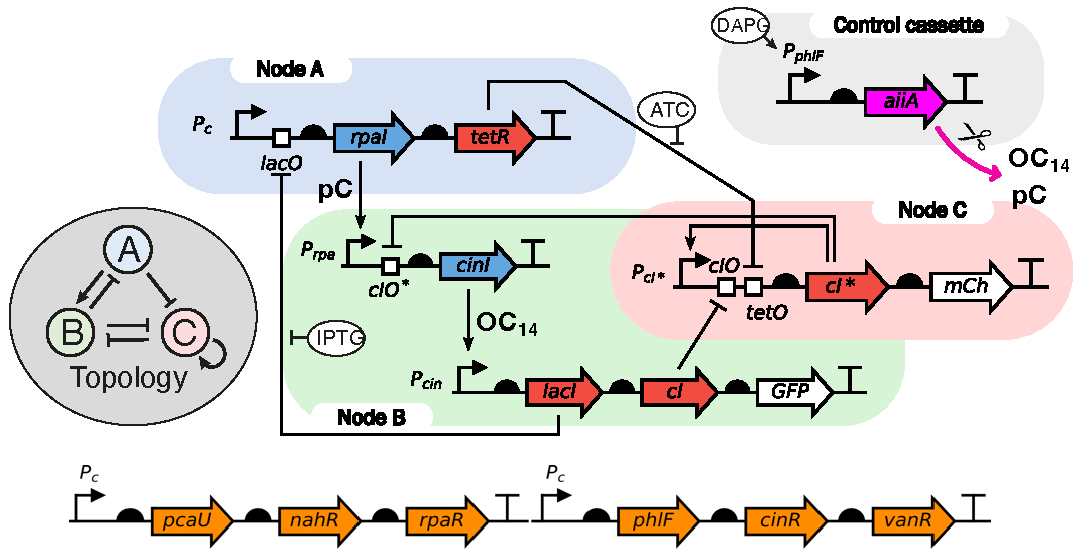
\includegraphics[width=1\textwidth]{chapters/Chapter 2/synthetic circuit2}
    \caption{\textbf{Synthetic biology implementation of \#1754 topology.} This synthetic circuit
    engineered by Dr.~Jure Tica and Tong Zhu is a genetic abstraction of the \#1754 topology in \cite{Scholes2019}.
    This circuit is transformed so every \textit{E.~coli} cell in the biofilm has a copy inside.
    The original topology (left, grey inset) has only three nodes, while the synthetic circuit (right) has six nodes.
    The six-gene circuit architecture, shown in standard notation, can be clustered into the three original nodes
    as seen by the blue, green and red bubbles.
    Diffusor synthesis enzymes, in blue, produce quorum sensing molecules $pC$ and $OC_{14}$ which diffuse out of the cell (blue and green arrows).
    Non-diffusible transcription
    factors (in red), also called repressor proteins, are lacI, cI, cI* and tetR.
    Fluorescent proteins GFP and mCherry are in white.
    The circuit can be regulated by small molecules aTc, IPTG and DAPG shown in white bubbles.
    DAPG activates the control cassette and produces regulated degradation of small quorum sensing molecules.
    The bottom cassette (orange), contains the necessary regulators:
    rpaR is the pC receptor (Node A diffusor), cinR is the OC14 receptor (Node B diffusor),
        and phlF is the DAPG receptor (used to tune inducible diffusor degradation).}
    \label{fig:synthetic circuit_chapter2}
\end{figure}

A \acrfull{PDE} system is used to describe the reaction and diffusion terms of this synthetic gene circuit (Fig.~\ref{fig:synthetic circuit_chapter2}).
This system of equations describes the concentration of molecules which are the dependent variables, in time and space which are the independent variables.
The molecules modelled are the six regulator genes and two diffusor molecules.
Diffusor molecules act as morphogens in this RD circuit.
This model includes:
\begin{itemize}
    \item Constant background production due to promoter leakiness
    \item Activator-repressor regulated gene expression using non-linear sigmoidal Hill terms
    \item Linear degradation of proteins and diffusor molecules or morphogens
    \item Diffusion of morphogens in a ~\acrfull{2D} space
    \item Effect of tuning molecules aTc, IPTG and DAPG on the circuit and diffusion
    \end{itemize}
The dynamics of a generic protein (X) and generic morphogen  (U) of the gene circuit, which are regulated by the activator [A] and inhibitor [I], are modelled in 2D as

\begin{subequations}\label{eq:Generalised protein and diffuser pde}
\begin{equation}
    \pdv{[X]}{t}= b_{X}+V_{X}\cdot\frac{1}{1+\left(\frac{K{A}}{[A]}\right)^{n_{A}}}\cdot\frac{1}{1+\left(\frac{[I]}{K_{I}}\right)^{n_{I}}}-\mu_{X}\cdot[X]
    \label{eq:Generalised protein}
\end{equation}

\begin{equation}
    \pdv{[U]}{t} = k_{1}\cdot[A] - \mu_{U}\cdot[U] + D_{U}\nabla^2 [U]
    \label{eq:generalised diffuser}
\end{equation}
\end{subequations}

This results in a PDE model with eight equations that correspond to the two diffusors
(pC and OC14) and six protein species of the circuit:
RpaI, CinI, TetR, LacI, cI* and cI.
This PDE model is reduced to a six-equation system by assuming a quasi-steady state for the diffusors,
with production and degradation kinetics much faster than those of proteins.
Finally, the model is non-dimensionalised to enable its parametrisation using liquid culture dose-response data.
This non-dimensionalisation involves tranaforming the model so the variables are expressed in terms of dimensionless units instead of concentration units.
In the subsections below, the different terms of Eq.~\ref{eq:Generalised protein and diffuser pde} are discussed.
Furthermore, the process of model reduction, non-dimensionalisation and fitting is also described.


\subsection{Protein equations and gene regulation}\label{Protein equations and gene regulation}
The rate of protein production can be defined as
\begin{equation}
    V = V_{max} \cdot \theta([X])
    \label{eq: vmax}
\end{equation}
where $\theta$ is a function of a generic protein X concentration which represents the fractional activation of the system.
Full activation of protein production is denoted as $\theta=1$ while full inhibition is represented by $\theta=0$.
$V_{\max}$ is the maximal rate of expression.
$\theta$ can be represented by a Hill function and an inverse-Hill function to describe cooperative binding,
derived using the law of mass action with all-or-none binding to multiple binding sites ~\parencite{Weiss1997}.
We further apply the quasi-steady state assumptions for activator and inhibitor binding to the promoter,
as well as for the mRNA dynamics,
as these timescales are much faster than protein production ~\parencite{Andersen1998, Bremer2008}.
This leads to the following expression of $\theta$ for non-competitive activation (A) and inhibition (I)
\begin{equation}
    \theta([A],[I])= \frac{1}{1+\left(\frac{K_{A}}{[A]}\right)^{n_{A}}} \cdot \frac{1}{1+\left(\frac{[I]}{K_{I}}\right)^{n_{I}}}
    \label{eq:theta}
\end{equation}
This Hill function is used in the Eq.~\ref{eq:Generalised protein} and describes promoter activity as a function of the two inputs [A] and [I], where $K_{A}$ and $K_{I}$ are half-activation/inhibition concentrations, $n_{A}$ and $n_{I}$ are the Hill coefficients.
Additionally, most promoters are leaky,
which we account for by introducing a small rate of background production $b_{X}$.
corresponds to the first term in Eq.~\ref{eq:Generalised protein}

\begin{figure}[H] % h! is a placement specifier; it tries to place the image here.
    \centering
    \begin{adjustbox}{center}
        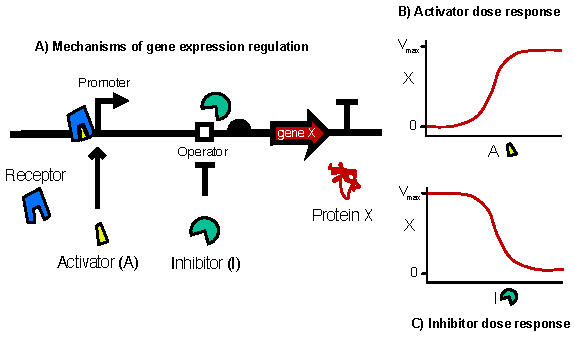
\includegraphics[width=1\textwidth]{chapters/Chapter 2/activation_inhibition2} % The name of your image file; assumes it is in the same directory as your .tex file
    \end{adjustbox}
    \caption{\textbf{Activation and Inhibition of gene expression.} \textbf{(A)} Mechanisms of gene expression regulation:
    The activator molecule (yellow) binds a receptor (blue),
        and this complex binds the promoter to activate gene expression.
    The inhibitor (green) binds the operator and inhibits gene expression.
    In the case of this model, activators are diffusors (pC, $OC_{14}$) with their respective receptors (RpaR, CinR) and inhibitors are proteins (RpaI, CinI, TetR, LacI, cI, cI*).
    \textbf{(B)} Expression of X dependent on activation by A modelled with a Hill function.
    \textbf{(C)} Expression of X dependent on inhibition by I modelled with an inverse-Hill function.}
    \label{fig:activation_inhibition} % A label for referencing this figure later in the document
\end{figure}

A visual representation of the mechanisms of activation and inhibition
modelled in Eq.~\ref{eq:theta} can be observed in Fig.~\ref{fig:activation_inhibition}.
Using Eq.~\ref{eq: vmax} and Eq.~\ref{eq:theta}, activator and inhibitor dose curves are be generated
(Fig.~\ref{fig:activation_inhibition}B-C).
These dose-response curves show the relationship between the activator or inhibitor and the rate of production of protein X.
Steeper curves are generated with higher cooperativity constants,
which are typical of cooperative systems where multiple transcription factors (TFs) can bind simultaneously.
These steep curves resemble electrical engineering circuits,
which use step functions instead of dose-response curves,
meaning a specific inducer concentration will drive the system from 0 to $V_{\max}$.
Finally,
the K parameter in Eq.~\ref{eq:theta} corresponds to the concentration of inducer
required to reach production of X at  $1/2 V_{\max}$.


\subsection{Tuning gene expression: aTc regulation of TetR and IPTG regulation of LacI}
Experimentally, the circuit was designed to be tuned in a variety of ways using aTc, IPTG and DAPG.
This tuning was used to achieve parameter combinations that are more favourable for patterning.
The following section introduces aTc and IPTG tuning into the model.

\begin{figure}[H] % h! is a placement specifier; it tries to place the image here.
    \centering
    \begin{adjustbox}{center}
        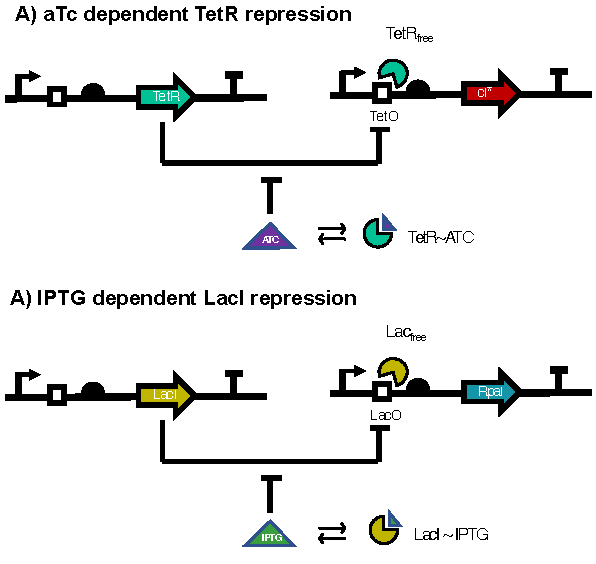
\includegraphics[width=0.7\textwidth]{chapters/Chapter 2/inducers} % The name of your image file; assumes it is in the same directory as your .tex file
    \end{adjustbox}
    \caption{\textbf{aTc and IPTG dependent repressions.}
    \textbf{(A)} TetR represses cI* by binding the TetO operator sequence.
    This repression can be inhibited by competitive binding of aTc to TetR.
    \textbf{(B)} LacI repression of RpaI* is inhibited by IPTG through competitive binding to LacI.}
    \label{fig:inducers} % A label for referencing this figure later in the document
\end{figure}

As shown in Fig.~\ref{fig:inducers}A, aTc binds to TetR and inactivates it.
Only free, unbound TetR can bind TetO and inactivate the expression of cI*.
The binding of aTc to TetR is modelled by a reversible equilibrium.
The affinity of binding is given by the $k_{on}$ and $k_{off}$ rate constants.

\begin{equation}
    aTc + TetR_{free} \xrightleftharpoons[k_{off}]{k_{on}} TetR \mhyphen aTc
\end{equation}

The law off mass action where the rate of reaction is the rate
constant multiplied by the concentration of reactants is applied.
Additionally, because this equilibrium happens at much faster rates than the protein production and degradation reactions of the model.
For this reason, quasi-steady state, which is valid when the system reaches equilibrium, is assumed

\begin{equation}
    \pdv{TetR \mhyphen aTc}{t} = k_{on}[TetR_{free}][aTc]^{n_{aTc}} - k_{off}[TetR \mhyphen aTc] \approx 0
\end{equation}


By rearranging terms and using $K_{D} = k_{off}/k_{on}$, a simplified expression for $[TetR_{free}]$ is obtained,
which is then used in the model

\begin{equation}
[TetR_{free}] = K_{D}\cdot \frac{[TetR \mhyphen naTc]}{[aTc]^{n_{aTc}}}
\end{equation}

Considering TetR is either free or bound to aTc, $[TetR-naTc]$ can be expressed as

\begin{equation}
[TetR \mhyphen naTc] = [TetR_{total}] - [TetR_{free}]
\end{equation}

to obtain the following expression

\begin{subequations}
    \begin{equation}
    [TetR_{free}] = K_{D} \cdot \frac{[TetR_{total}] - [TetR_{free}]}{[aTc]^{n_{aTc}}} \Longrightarrow
    \end{equation}
    \begin{equation}
    [TetR_{free}] (1+\frac{K_{D}}{[aTc]^{n_{aTc}}}) = \frac{K_{D}\cdot [TetR_{total}]}{[aTc]^{n_{aTc}}}\Longrightarrow
    \end{equation}
    \begin{equation}
    [TetR_{free}] = \frac{K_{D}\cdot[TetR_{total}]}{[aTc]^{n_{aTc}}+K_{D}} = \frac{[TetR_{total}]}{1+\frac{[aTc]^{n_{aTc}}}{K_{D}}}
    \end{equation}
\end{subequations}

which says that the concentration of unbound TetR is given by ~$[aTc]$,
~$[TetR_{total}]$ and the equilibrium constant ~$K_{D}$.

For non-cooperative systems where ~$n=1$, ~$K_{D}=[L_{half}]$, where $[L_{half}]$ is the $[aTc]$ at half repression.
However, for cooperative systems where ~$n>1$, ~$[L_{half}] = \sqrt[n]{K_{D}}$.
We define a new variable ~$K_{A} = \sqrt[n]{K_{D}} \leftrightarrow K_{D} = K^n_{A}$
that we use to replace ~$K_{D}$ in the following expression,
where $K^n_{A}$ is written as $K_{TetR \mhyphen aTc}$.
This was also done for other ~$K_{D}$ parameters of the model.
\begin{equation}
[TetR_{free}] =  \frac{[TetR_{total}]}{1+(\frac{[aTc]}{K_{TetR \mhyphen aTc}})^{n_{aTc}}}
\end{equation}
Parameter $K_{TetR \mhyphen aTc}$ is the dissociation constant of aTc to TetR,
whereas $n_{aTc}$ is the cooperativity of TetR and aTc binding.
This expression for unbound TetR ($[TetR_{free}]$ ), can then be introduced into the production rate of cI*.
cI* has an operator sequence downstream of the promoter, TetO.
This TetO is bound by TetR to inhibit the expression of the mRNA.
We will model the production of cI* dependent on TetR binding,
using an inverse-Hill term
that describes repression by this binding as described by Eq.~\ref{eq: vmax} and Eq.~\ref{eq:theta}.

\begin{equation}
    \pdv{[cI*]}{t} = V_{max}\cdot \left(1+\left(\frac{[TetR_{free}]}{K_{TetR \mhyphen TetO}}\right)^{n_{TetO}}\right)^{-1} = V_{max} \cdot \left(1+\left(\frac{TetR_{total}}{K_{TetR \mhyphen TetO}\cdot(1+(\frac{aTc}{K_{TetR \mhyphen aTc}})^{n_{aTc}})}\right)^{n_{TetO}}\right)^{-1}
\end{equation}

We can simplify the denominator so

\begin{equation}
    \pdv{[cI*]}{t} = V_{max}\cdot \left(1+\left(\frac{[TetR_{total}]}{K_{TetR \mhyphen TetO \mhyphen aTc }}\right)^{n_{TetO}}\right)^{-1}
\end{equation}

where

\begin{equation}
    K_{TetR \mhyphen TetO \mhyphen aTc}=K_{TetR \mhyphen TetO}\cdot(1+(\frac{aTc}{K_{TetR \mhyphen aTc}})^{n_{aTc}})
\end{equation}

The parameter $K_{TetR \mhyphen TetO \mhyphen aTc}$ is the dissociation constant of TetR to TetO (which in our model is aTc dependent), $K_{TetR \mhyphen aTc}$
is the affinity of aTc to TetR, $n_{aTc}$ is the Hill coefficient of aTc and TetR,
and $n_{TetO}$ is the Hill coefficient of TetR to TetO.
Therefore, the higher the aTc, the higher the production of cI*, which is the transcription factor repressing node B.

The same logic can be applied for the IPTG regulating LacI inhibition (see Fig.~\ref{fig:inducers}B),
where unbound LacI can be or $[LacI_{free}]$ can be expressed as
\begin{equation}
[LacI{free}] =  \frac{[LacI_{total}]}{1+(\frac{[IPTG]}{K_{LacI \mhyphen IPTG}})^{n_{IPTG}}}
\end{equation}

LacI-free will be then able to bind to LacO and inhibit RpaI and TetR production in the following manner

\begin{equation}
    \pdv{[RpaI]}{t} = V_{max}\cdot \left(1+\left(\frac{[LacI_{free}]}{K_{LacI \mhyphen LacO}}\right)^{n_{LacO}}\right)^{-1} = V_{max} \cdot \left(1+\left(\frac{LacI_{total}}{K_{LacI \mhyphen LacO}\cdot(1+(\frac{IPTG}{K_{LacI \mhyphen IPTG}})^{n_{IPTG}})}\right)^{n_{LacO}}\right)^{-1}
\end{equation}


We can again simplify the denominator so

\begin{equation}
    \pdv{[RpaI]}{t} = V_{max}\cdot \left(1+\left(\frac{[LacI_{total}]}{K_{LacI \mhyphen LacO \mhyphen IPTG }}\right)^{n_{LacO}}\right)^{-1}
\end{equation}

where,

\begin{equation}
    K_{LacI \mhyphen LacO \mhyphen IPTG} = K_{LacI \mhyphen LacO}\cdot(1+(\frac{IPTG}{K_{LacI \mhyphen IPTG}})^{n_{LacO}})
\end{equation}

The parameter $K_{LacI \mhyphen LacO \mhyphen IPTG}$ is the dissociation constant of TetR to TetO, $K_{LacI \mhyphen IPTG}$
is the affinity of IPTG to LacI, $n_{IPTG}$ is the Hill coefficient of IPTG and LacI,
and $n_{LacO}$ is the Hill coefficient of LacI to LacO.
Therefore, the higher the IPTG, the higher the production of RpaI, which is the synthesis enzyme producing pC to activate node B.




\subsection{Degradation}
All the species of the circuit, including proteins and diffusors,
were modelled to undergo linear, or first order, degradation
\begin{equation}
    -\mu_{P_{1}}[X]
    \label{linear degradation}
\end{equation}


as seen in Eq.~\ref{eq:Generalised protein and diffuser pde}.
The degradation rate parameters for the protein species and diffusors are readily available in the literature~\parencite{Andersen1998, kaufmann2005revisiting}
and can be found in Table~\ref{table:degradation table}.
They are scale-free parameters that only depend on time,
which makes them more translatable between different experimental contexts and units of measurement.



\begin{table}[H]
    \centering
    \begin{tabular}{|c|c|c|}
        \hline
        \textbf{Degradation tag} & \textbf{Molecule} & \textbf{Rate $[h^{-1}]$} \\
        \hline
        LVA 1 & CinI, LacI, cI, cI*, TetR 1 & 1.14 \\
        \hline
        ASV & RpaI, GFP, mCherry 3 & 0.30 \\
        \hline
        diffusors & pC, $OC_{14}$ & 0.0225 \\
        \hline
    \end{tabular}
    \caption{\textbf{Degradation Parameters.} Degradation coefficients of protein species with degradation tags LVA and ASV, and basal degradation of diffusors.}
    \label{table:degradation table}
\end{table}

The proteins of the circuit had short peptide sequences added at their 3’ ends,
known as degradation tags, that promote their breakdown by the cell’s proteolytic enzymes.
The diffusor's degradation could be further induced
by adding exogenous DAPG to the system which induces degradation by AiiA lactonase.

\subsection{Diffusor equations}
Diffusors ($pC$ and $OC_{14}$) are synthesised by enzymes (rpaI and cinI), and then bound to receptors (rpaR and cinR) to activate gene expression by binding to the promoters (Prpa and Pcin)
 as seen Fig.~\ref{fig:activation_inhibition}.
The circuit receptors are expressed constructively from a low-copy pCC1 plasmid,
and are therefore modelled with a constant concentration.
The quasi-steady state was assumed for the very fast equilibrium that forms between the receptor and the diffusors.
The receptor-inducer and receptor-promoter binding equilibria were modelled with mass action kinetics.

The enzymatic production of the diffusors was modelled with a simple linear production term dependent on synthesis enzyme concentration
([A], [B]),
and a rate constant
($K_{1}$ and $K_{2}$).
It is assumed that the precursor substrate concentration is in excess and does not influence the reaction rate.


The diffusors are also modelled to undergo linear degradation,
parameterised by $\mu_{U}$ and $\mu_{V}$ as seen in Eq.~\ref{linear degradation}.
This degradation is a combination of spontaneous hydrolysis in water, enzymatic AiiA-dependent degradation,
and other cellular metabolic processes ~\parencite{kaufmann2005revisiting,Wang2004,Momb2008}.
Finally,
the diffusor movement through space is modelled with simple diffusion terms and parameterised with diffusion coefficients $D_{U}$ and $D_{V}$.

\begin{subequations}\label{diffuser}
\begin{equation}
    \pdv{[U]}{t} = k_{1}\cdot[A] - \mu_{U}\cdot[U] +  D_{U}\nabla^2 [U]
\end{equation}
\begin{equation}
    \pdv{[V]}{t} = k_{2}\cdot[B] - \mu_{V}\cdot[V] + D_{V}\nabla^2 [V]
\end{equation}
\end{subequations}

The time dynamics of diffusor synthesis are much faster than that of protein production.
Therefore, the rate of change of diffusors is expected to be much higher than that of proteins.
These rapid fluctuations of diffusors can be approximated to equilibrium by using the quasi-steady state approximation,
meaning the rate is set to zero.
This leads to an expression of diffusor concentration
that is linearly correlated with their synthesis enzyme and rate constant,
and inversely correlated with their degradation rate.

\begin{subequations}\label{diffuser quasi-steady state}

\begin{equation}\label{diffU}
    \pdv{[U]}{t} = k_{1}\cdot[A] - \mu_{U}\cdot[U] = 0
    \longrightarrow U = \frac{k_{1}}{\mu_{U}}[A]
\end{equation}

\begin{equation}\label{diffV}
    \pdv{[V]}{t} = k_{2}\cdot[B] - \mu_{V}\cdot[V] = 0
    \longrightarrow V = \frac{k_{2}}{\mu_{V}}[B]
\end{equation}
\end{subequations}

In this process, the diffusion of U and V is artificially assigned to A and B, since

\begin{subequations}\label{[diffuser_artificial]}

\begin{equation}
    U = \frac{k_{1}}{\mu_{U}}[A] \longrightarrow D_{U}
    \nabla^2 [U] = D_{U}\frac{k_{1}}{\mu_{U}}  \nabla^2  [A]\label{eq:equation2}
\end{equation}

\begin{equation}
    V = \frac{k_{2}}{\mu_{V}}[B] \longrightarrow D_{V}
    \nabla^2 [V] =  D_{V}\frac{k_{2}}{\mu_{V}}  \nabla^2  [B]\label{eq:equation}
\end{equation}

\end{subequations}

These quasi-steady state expressions are used to model the diffusors implicitly within the gene equations.
Therefore, instead of using eight equations for the six genes and two diffusors;
we have six equations for the six genes with the two diffusors modelled implicitly.
This
U and V will be modelled within A and B in the Hill activation and diffusion terms

\begin{equation}\label{8to6A}
    \pdv{[A]}{t} = b_{A}+V_{A}\cdot \frac{1}{\left(1+\left(\frac{[I]}{K_{I}}\right)^{n_{I}}\right)}-\mu_{A}\cdot[A] + \frac{k_{1}D_{U}}{\mu_{U}}\cdot \nabla^2 [A]
\end{equation}

\begin{equation}\label{8to6B}
    \pdv{[B]}{t} = b_{B}+V_{B}\cdot\frac{1}{1+\left(\frac{\mu_{u}K{ub}}{k_{1}[A]}\right)^{n_{ab}}}\cdot\frac{1}{1+\left(\frac{[I]}{K_{I}}\right)^{n_{I}}}-\mu_{B}\cdot[B] + \frac{k_{2}D_{V}}{\mu_{V}}\cdot \nabla^2 [B]
\end{equation}

This simplification is taken to convert the model from an 8 equation to a 6 equation model, to reduce the computational requirements.
We assume this is possible as because of the linear relationship between diffuser and synthesis enzymes.
However, it is important to note that Eqs.~\ref{8to6A},~\ref{8to6B} are derived from the phenomenological nature of the circuit rather than rationally from the equations.

\subsection{Six-equation model}
We combined all the terms described above including basal production,
activator or inhibitor-regulated production, tuning molecules, linear degradation and implicit diffusors.
All these terms are applied to the circuit shown in Fig~\ref{fig:synthetic circuit_chapter2}.
This results in a six-equation model with information on the six proteins in space and time

\begin{subequations}\label{[6 equation proteins]}

\begin{equation}
    \pdv{[A]}{t} = b_{A}+V_{A}\cdot \frac{1}{\left(1+\left(\frac{[D]}{K_{da}}\right)^{n_{da}}\right)}-\mu_{A}\cdot[A] + \frac{k_{1}D_{U}}{\mu_{U}}\cdot \nabla^2 [A]
\end{equation}

\begin{equation}
    \pdv{[B]}{t} = b_{B}+V_{B}\cdot\frac{1}{1+\left(\frac{\mu_{u}K{ub}}{k_{1}[A]}\right)^{n_{ab}}}\cdot\frac{1}{1+\left(\frac{[E]}{K_{eb}}\right)^{n_{eb}}}-\mu_{B}\cdot[B] + \frac{k_{2}D_{V}}{\mu_{V}}\cdot \nabla^2[B]
\end{equation}

\begin{equation}
    \pdv{[C]}{t} = b_{C}+V_{C}\cdot \frac{1}{\left(1+\left(\frac{[D]}{K_{da}}\right)^{n_{da}}\right)}-\mu_{C}\cdot[C]
\end{equation}

\begin{equation}
    \pdv{[D]}{t} = b_{D}+V_{D}\cdot\frac{1}{1+\left(\frac{\mu_{V}K{vd}}{k_{2}[B]}\right)^{n_{bd}}}-\mu_{D}\cdot[D]
\end{equation}

\begin{equation}
    \pdv{[E]}{t} = b_{E}+V_{E}\cdot \frac{1}{\left(1+\left(\frac{[C]}{K_{ce}}\right)^{n_{ce}}\right)}\cdot\frac{1}{1+\left(\frac{[F]}{K_{fe}}\right)^{n_{fe}}}\cdot\frac{1}{1+\left(\frac{K{ee}}{[E]}\right)^{n_{ee}}}-\mu_{E}\cdot[E]
\end{equation}

\begin{equation}
    \pdv{[F]}{t} = b_{F}+V_{F}\cdot\frac{1}{1+\left(\frac{\mu_{V}K_{bd}}{k_{2}[B]}\right)^{n_{bd}}}-\mu_{F}\cdot[F]
\end{equation}

\end{subequations}

where $K_{da}$ and $K_{ce}$ are expressed in terms of the tuning molecules such as

\begin{subequations}
    \begin{equation}\label{kda_iptg}
        K_{da} = K_{lacI-lacO} \left( 1 + \frac{[IPTG]}{K_{lacI-IPTG}}\right)^{n_{IPTG}}
    \end{equation}

    \begin{equation}\label{kce_atc}
        K_{ce} = K_{tetR-tetO} \left( 1 + \frac{[aTc]}{K_{tetR-aTc}}\right)^{n_{aTc}}
    \end{equation}
\end{subequations}

The six dependent variables can be found in Table~\ref{tab:Model variables}.
They can be thought of as protein concentrations,
although they are also directly linked to the gene expressed to produce that protein.
The units are nM.
\begin{table}[H]
    \centering
    \caption{\textbf{Model dependent variables.} The model-dependent variables are the concentrations of the six regulatory proteins.
    The names of the molecule and the original node they belong to in the original \#1754 topology are also shown.}
    \label{tab:Model variables}
    \renewcommand{\arraystretch}{1.3} % Adjust vertical padding
    \begin{tabular}{|c|c|c|}
        \hline
        \textbf{Variable} & \textbf{Biological molecule} & \textbf{Node in original 3-node circuit}\\
        \hline
        [A] & RpaI & A\\
        \hline
        [B] & CinI & B \\
        \hline
        [C] & TetR & A\\
        \hline
        [D] & LacI & B \\
        \hline
        [E] & cI* & C \\
        \hline
        [F] & cI & B \\
        \hline
    \end{tabular}
\end{table}
A description of the parameters used in the model can be found in Table~\ref{tab:model params}.

\begin{table}[H]
    \centering
    \caption{\textbf{Model parameters, description and units}}
    \label{tab:model params}
    \renewcommand{\arraystretch}{1.3} % Adjust vertical padding
    \begin{tabular}{|c|c|c|}
        \hline
        \textbf{Parameter} & \textbf{Description} & \textbf{Units}\\
        \hline
        $t$ & Time & h\\
        \hline
        $x$ & Space & mm\\
        \hline
        $b_{X}$ & Background production rate of X & nM/h\\
        \hline
        $V_{X}$ & Induced max production rate of X & nM/h \\
        \hline
        $K_{XY}$ & Dissociation constant of X binding to Y regulator DNA & nM \\
        \hline
        $n_{XY}$ & Cooperativity constant of X binding to Y regulator DNA & 1\\
        \hline
        $\mu_{X}$ & Degradation rate of X & 1/h\\
        \hline
        $D_{X}$ & Diffusion rate of diffusor X & $mm^2/h$\\
        \hline

    \end{tabular}
\end{table}


For $K_{XY}$ and $n_{XY}$,
activators X will bind to a receptor molecule that binds the promoter sequence upstream of gene Y;
while inhibitor X will bind to the operator sequence upstream of gene Y.



\subsection{Dimensionless six-equation model}

A dimensionless model (or non-dimensional model) is derived to better understand the nature of the parameters,
and to simplify the fitting process, as explained below.
The work on transforming the six-equation model into a non-dimensional form was done in collaboration with Dr.~Roozbeh Pazuki.
The non-dimensionalisation involves the following transformations of dependent and independent variables of concentration
(X),
time (t) and space
(x and y).


\begin{equation}\label{variable transformations}
    X = \frac{b_{x}}{\mu_{x}}X^*, t = \frac{t^*}{\mu_{a}},
    x = \sqrt{\frac{k_{1}D_{u}}{\mu_{a}\mu_{u}}}x^*, y = \sqrt{\frac{k_{1}D_{u}}{\mu_{a}\mu_{u}}}y^*
\end{equation}

and the following transformations of the system parameters V, µ, K and D:

\begin{equation}\label{parameter transformations}
    V_{x}^*=\frac{V_{x}}{b_{x}},  \mu_{x}^* = \frac{\mu_{x}}{\mu_{a}},
K^*_{yx} = \frac{\mu_{x}}{b_{x}}K ,D_{r} = \frac{k_{2}D_{v}\mu_{u}}{k_{1}D_{u}\mu_{v}}
\end{equation}

It is important to note that time and degradation of all species is now relative to the degradation rates of A
(RpaI) which is an estimated parameter from the literature
(see Table~\ref{table:degradation table}).
If this parameter changes throughout the experiment, the effects should be absorbed by the dimensionless model.
If those transformations are applied to the original six-equation model shown in Eqs.~\ref{[6 equation proteins]}, the following dimensionless model is obtained

\begin{subequations}\label{six_eq_dimensionless}

    \begin{equation}
        \pdv{[A^*]}{t^*} = 1 + V_{a}^* \left(\frac{1}{1+\left(\frac{[D^*]}{K_{da}^*}\right)^{n_{da}}}\right) - [A^*] + \nabla^2 [A^*]
    \end{equation}

    \begin{equation}
        \pdv{[B^*]}{t} =\mu_{b}^* \left(1+V_{B}^*\left(\frac{1}{1+\left(\frac{\mu_{u}K{ub}^*}{k_{1}[A^*]}\right)^{n_{ab}}}\right)\cdot\left(\frac{1}{1+\left(\frac{[E^*]}{K_{eb}^*}\right)^{n_{eb}}}\right) -[B^*] \right)+ D_{r}\nabla^2 [B^*]
    \end{equation}

    \begin{equation}
        \pdv{[C^*]}{t^*} = \mu_{c}^*\left(1 + V_{c}^* \left(\frac{1}{1+\left(\frac{[D^*]}{K_{da}^*}\right)^{n_{da}}}\right) - [C^*]\right)
    \end{equation}

    \begin{equation}
        \pdv{[D^*]}{t^*} = \mu_{d}^*\left(1 + V_{d}^* \left(\frac{1}{1+\left(\frac{\mu_{v}K_{vd}^*}{k_{2}[B^*]}\right)^{n_{vd}}}\right) - [D^*]\right)
    \end{equation}
    \begin{equation}
        \pdv{[E^*]}{t^*} = \mu_{e}^*\left(1 + V_{e}^* \left(\frac{1}{1+\left(\frac{[C^*]}{K_{ce}^*}\right)^{n_{ce}}}\right)\left(\frac{1}{1+\left(\frac{[F^*]}{K_{fe}^*}\right)^{n_{fe}}}\right)\left(\frac{1}{1+\left(\frac{K_{ee}^*}{[E^*]}\right)^{n_{ee}}}\right)  - [E^*]\right)
    \end{equation}
    \begin{equation}
        \pdv{[F^*]}{t^*} = \mu_{f}^*\left(1 + V_{f}^* \left(\frac{1}{1+\left(\frac{\mu_{v}K_{vd}^*}{k_{2}[B^*]}\right)^{n_{vd}}}\right) - [F^*]\right)
    \end{equation}

\end{subequations}

A summary of the model parameters including notation,
original units and dimensionless units can be found in Table~\ref{tab:Dimensionless_params}.


\begin{table}[H]
    \centering
    \caption{\textbf{Dimensionless model parameters and unit transformations}}
    \label{tab:Dimensionless_params}
    \renewcommand{\arraystretch}{2.3} % Adjust vertical padding
    \begin{tabular}{|c|c|c|c|}
        \hline
        \textbf{Parameter} & \textbf{Description} & \textbf{Original Units} & \textbf{Dimensionless Units} \\
        \hline
        $X^*$ & Molecular species & $nM$ & $\frac{\mu_{x}}{b_{x}}X \quad \rightarrow \quad  \frac{nM/h}{nM/h}  = 1$
        \\
        \hline

        $OC_{14}$ & NodeB inducer & $nM$ & $\frac{k_{2} b_{B}}{\mu_{v} \mu_{b}} B^* \quad \rightarrow \quad  1$
        \\
        \hline
        $b_{x}^*$ & Background production rate & $nM/h$ & no $b_{x} $\\
        \hline
        $ V_{x}^*$  & Induced max production rate & $nM/h$ & $ \frac{V_{x}}{b_{x}} \quad \rightarrow \quad  \frac{nM/h}{nM/h} = 1 $\\
        \hline
        $K_{yx}^*$ & Dissociation constant & $nM$ & $ \frac{\mu_{x}}{b_{x}} K_{yx} \quad \rightarrow \quad \frac{nM/h}{nM/h} = 1 $\\
        \hline
        $ n_{yx}$  & Cooperativity constant & 1 & 1\\
        \hline
        $ \mu_{x}^* $ & Degradation rate & $1/h$ & $\frac{\mu_{x}}{\mu_{a}} \quad \rightarrow \quad  \frac{1/h}{1/h}=1 $\\
        \hline
        $D_{x}$ & Diffusion rate & $mm/h$ & $ \frac{k_{2} D_{v} \mu_{u}}{k_{1} D_{u} \mu_{v}} \quad \rightarrow \quad  1$  \\
        \hline
        $ t $ & Time & $h$ & $\mu_{a} \cdot t \quad \rightarrow \quad  h \cdot  h^{-1} =1$\\
        \hline
        $ x$  & Space & $mm$ & $\sqrt{\frac{k_{1} D_{1}}{\mu_{a}\mu_{v}}}/x \rightarrow  \sqrt{\frac{h^{-1} mm^{2} h^{-1}}{h^{-1}h^{-1}}}/mm  = 1$ \\
        \hline
    \end{tabular}
\end{table}

\subsection{Fluorescence reporters}
In addition to the six genes involved in circuit regulation, there are two fluorescent reporter genes: GFP and mCherry.
GFP is in the same operon as lacI and cI, meaning a single mRNA is transcribed with the three genes.
The difference is that each has its own Ribosome Binding Site (RBS),
so they are translated into proteins independently.
Therefore, we can assume GFP is linearly correlated with lacI and cI.
The same thing can be inferred for mCherry and cI*.
Instead of modelling GFP and mCherry as two extra equations,
lacI and cI* concentrations will be used instead when studying how the fluorescent distributions look spatially

\begin{subequations}
    \begin{equation}
        [GFP] = \alpha_{GFP}*[LacI]
    \end{equation}
    \begin{equation}
        [mCherry] = \alpha_{mCherry}*[cI^*]
    \end{equation}
    \label{linear_fluorescence}
\end{subequations}

where $\alpha$ is the fractional translation between the two proteins in the same operon.


Both the dimensional and the non-dimensional six-equation models
(Eqs.~\ref{[6 equation proteins]} and Eqs.~\ref{six_eq_dimensionless})
are a close representation of the synthetic gene circuit engineered
by~\cite{Tica2020} shown in Fig.~\ref{fig:synthetic circuit_chapter2}.
The non-dimensional model (Eqs.~\ref{six_eq_dimensionless})
will be used to explore the potential of this gene circuit for pattern formation by studying GFP and mCherry distributions in an \textit{in-silico} model tissue.



\section{Explore parameter space and optimise robustness}
Before performing any experiments on the gene circuit,
the parameter space of our system was explored
to understand which possible spatio-temporal dynamics could be generated by this circuit.
In particular, it was studied
whether this six-node synthetic biology implementation of the original three-node network from~\cite{Scholes2019} (Fig.~\ref{fig:synthetic circuit_chapter2}) could produce Turing patterns.
Finally, the parameter space was explore to understand how to tune the genetic circuit experimentally to maximise the likelihood of Turing pattern formation.
Two approaches were taken
which include
investigating the effects of matching dose-response curves to increase Turing robustness
and understanding the effects of individual parameters on Turing robustness.

\subsection{Definition of parameter space based on literature parameters}\label{Definition of parameter space based on literature parametrisation}
The model is first studied by initialising the model parameters from distributions derived from the literature.
This multi-dimensional distribution enables a full understanding of the gene circuit behaviour in all possible parameter regimes.
A distribution for each parameter was generated,
and the multi-dimensional parameter space was sampled using Latin Hypercube Sampling
(see~\ref{sampling method})~\parencite{Iman2014, Bergstra2012},
which maximises the sampling efficiency with fewer samples.
Depending on the uncertainty of the parameter, different distributions were used such as Loguniform, Gaussian and Fixed.
 For each parameter of the model,
literature searches were carried out to define biologically realistic lower and upper bounds.
Diffusion rates~($D$) were estimated in unpublished data~\parencite{tica_diffusers}.
Diffusor production rate constants ($k$) in~\cite{Schaefer1996, Pai2009}.
Protein degradation rates in~\cite{Andersen1998}, while diffusor degradation in~\cite{kaufmann2005revisiting}.
Cooperativity values ($n$) in~\cite{Babic2007}.
Other parameters that had not been well parametrised in the literature were defined with bounds such as the maximum production rate
($V_{X}$),
background production rate ($b_{X}$) and Dissociation constant
($K_{XY}$).
Although we have less confidence in these last parameter estimations,
bounds were still obtained from the literature ~\parencite{Scholes2019, Pusnik2019}.
The types of distributions
used for sampling and the values used for each parameter are listed in Table~\ref{tab:literature param distributions}.
To obtain dimensionless parameters from these, the bounds of the distributions are recalculated,
and the distributions sampled between these new bounds as specified in the ‘Distribution’
column of Table~\ref{tab:literature param distributions}.
The transformations
required to get the dimensionless bounds or values can be found in Eq.~\ref{variable transformations} and Eq.~\ref{parameter transformations} or Table~\ref{tab:Dimensionless_params}.
For example, for Dr* which is $(k_{2}D_{v}\mu_{u})/(k_{1}D_{u}\mu_{v})$,
a loguniform distribution was sampled between new bounds [0.01, 100].
\begin{table}[H]
    \caption{\textbf{Literature-derived parameter distributions.} The distributions used include Loguniform and Gaussian.
    Some parameters are fixed to single values and not sampled.
    The parameters shown here are dimensional, so these distributions are then used in the dimensionless form of parameters shown in Eq.~\ref{variable transformations} and Eq.~\ref{parameter transformations}.}
\label{tab:literature param distributions}
\renewcommand{\arraystretch}{1.3} % Adjust vertical padding
\begin{tabular}{|p{20mm}|p{57mm}|c|p{25mm}|}
\hline
\textbf{Parameter} & \textbf{Description} & \textbf{Distribution} & \textbf{Value}\\
\hline

$V_{X}$ & Induced max production rate of X & Loguniform &  10-1000 \\
\hline
$b_{X}$ & Background production rate of X & Loguniform & 0.1-1\\
\hline
$D_{U}, D_{V}$ & Diffusion rate of pC and $OC_{14}$ & Loguniform & 0.1-10\\
\hline
$K_{XY}$ & Dissociation constant of X binding to Y regulator DNA & Loguniform & 0.1-250\\
\hline
$K_{ee}$ & Dissociation constant of cI* binding its own promoter ($P_{cI*}$) & Fixed & 0.01\\
\hline
$k_{1},k_{2}$ & pC and $OC_{14}$ production rate constants  & Fixed & 0.0183\\
\hline
$\mu_{u},\mu_{v}$ & pC and $OC_{14}$ degradation rates & Fixed & 0.0225\\
\hline
$\mu_{LVA}$ & Degradation rates of proteins with LVA tag (CinI, LacI, cI, cI*, TetR $\rightarrow \mu_{B}, \mu_{C}, mu_{D}, \mu_{E}, \mu_{F}$) & Gaussian & mean=1.143, std=mean*0.1\\
\hline
$\mu_{ASV}$ & Degradation rates of proteins with LVA tag (RpaI $\rightarrow \mu_{A}$) & Fixed & 0.3\\
\hline
$n_{ub}, n_{vd}$ & Cooperativity of pC and $OC_{14}$ with receptors binding binding to $P_{rpa}$ and $P_{cin}$ promoters respectively & Fixed & [1,2]\\
\hline
$n_{da}$, $n_{fe}$, $n_{ee}$, $n_{eb}$, $n_{ce}$ & Cooperativity of LacI, cI, cI*, cI*, TetR binding to lacO, cIO, $P_{cI*}$, cIO*, tetO operators and promoter respectively & Fixed & [2,5,4,4,3]\\
\hline
\end{tabular}
\end{table}

\subsection{Finding Turing in six-node Turing circuit and defining robustness}
Linear stability analysis was used initially to understand whether the circuit built synthetically could produce Turing patterns.
By searching the parameter space defined above using linear stability analysis,
several diffusion-driven instabilities were found.
When simulated these gave rise to Turing patterns
varying from labyrinths to spots as seen in Fig.~\ref{fig:square_turing}.
Although the robustness is limited (as described later),
the synthetic gene circuit engineered by~\cite{Tica2020} can indeed produce stationary periodic patterns
resulting from a Turing mechanism.

\begin{figure}[H]
    \centering
    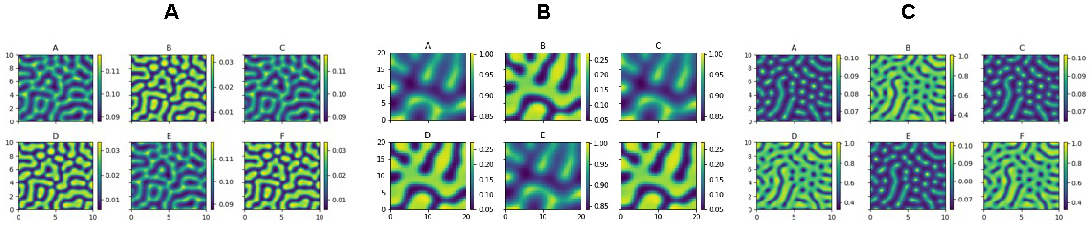
\includegraphics[width=1\textwidth]{chapters/Chapter 2/square_turing}
    \caption{\textbf{Examples of Turing patterns in the six-node circuit.} Three simulations of the six-equation model with Turing I parameter sets.
    In each solution (A, B, C) there are six images which represent every dependent variable of the model.
    The solver used is the \acrfull{ADI} method with non-growing square domains and reflecting boundary conditions.
    Periodic patterns are observed.}
    \label{fig:square_turing}
\end{figure}

\subsection{Increasing Turing robustness by matching consequent dose-response curves}\label{balancing}
One of the aims of the model is
to understand
how to increase the robustness for Turing pattern formation \textit{in-silico} before the experimental work.
This way, we can then use the insights to maximise the chances of finding Turing patterns \textit{in-vitro}.
In this thesis,
we describe Turing robustness as the volume of the parameter space leading to Turing I and Turing I Hopf patterns.
Turing I Hopf patterns are included in this definition as in the context of the six-equation model and the parameters used, they seem to always produce periodic stationary patterns.
This can be seen in the following chapter where we explore these solutions numerically (see Fig.~\ref{system_class_simulations}).

The first approach consisted in investigating how a well-balanced circuit improves the likelihood of patterning.
Once the components of the circuit are put together inside the cell,
these components might not necessarily match well together.
Gene circuits, as opposed to digital circuits, do not have binary inputs and outputs.
Instead, gene expression is regulated continuously,
where a continuous increase in inducer leads to a continuous change in protein concentration
as seen in the dose-response curves of Fig.~\ref{fig:balancing}A
(left).
In this case, inducer [A0*] determines how much [A1*] is produced with a sigmoidal relationship.
The dose-response function is modelled with Hill terms as seen in Eq.\ref{eq:theta}.
A well-matched transfer function occurs when the protein expression levels stemming from dose-response 1
(Fig.~\ref{fig:balancing}A (left))
are compatible with the sensitivity of the regulatory components they act on for dose-response 2
(Fig.~\ref{fig:balancing}A (right)).
For example, a transfer function is not ‘matched’
when a very sensitive promoter is completely turned on even with background levels of activator.
This can occur experimentally
if the background levels of the activator are sufficiently high because of a leaky promoter or strong RBS.
In this case, an induction of the activator above the background would not result in further activation,
leading to a loss of dynamic range (Fig.~\ref{fig:balancing}C (red)).


\begin{figure}[H]
    \centering
    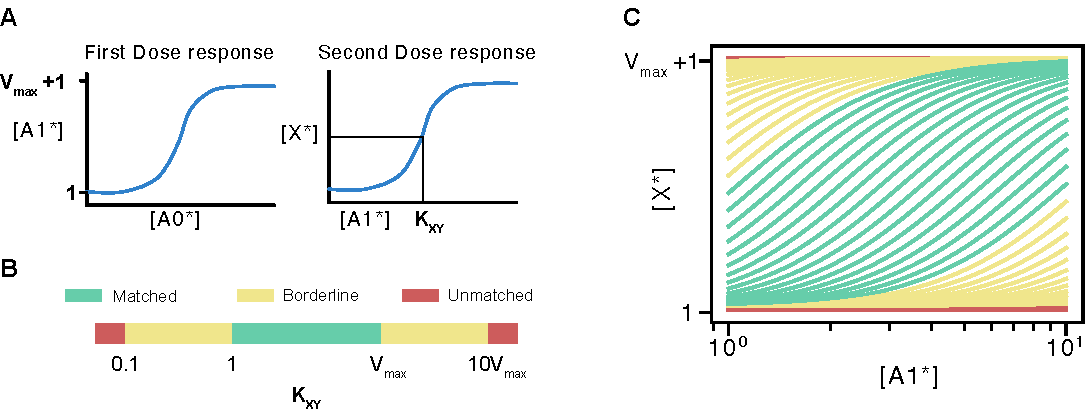
\includegraphics[width=1\textwidth]{chapters/Chapter 2/balancing}
    \caption{\textbf{Balancing of dose-response curves for an inducer-dependent activation.} \textbf{(A)} The first dose-response curve (left) describes the [A0*] dependent production of [A1*] which can vary from $1$ to $V_{\max}+1 $. [A1*], which is the output of the first dose-response, serves as an input for the second dose-response (right). The second dose-response curve describes the [A1*] dependent production of [X*]. The transfer function of the two dose-response curves is said to be balanced or matched if $K_{XY}$ is within the bounds [A1*]. \textbf{(B)} Diagram showing the values of parameter $K_{XY}$ from the second dose-response which generates unmatched (red), borderline matched (yellow), and matched (green) transfer functions. These parameters are with respect to $V_{\max}$ from the first dose-response. \textbf{(C)} Dose-response curves are generated with parameters from the three regions in (B). Matched dose-response curves (green) are the most sensitive to inducer, showing the biggest dynamic range.}
    \label{fig:balancing}
\end{figure}


Mathematically, to ensure a transfer function is matched,
the $K^*_{XY}$ of the second dose-response producing X needs
to be within the dynamic range of the dose-response 1 producing A1 as seen in Fig.~\ref{fig:balancing}A.
The lower bound is the steady state $[X^*]_{ss0}$ when the gene is completely turned off, $\theta=0$.
The upper bound is the steady state $[X^*]_{ss1}$ when the gene is completely turned on, $\theta=1$.
The two bounds can be obtained
by replacing $\theta$ by 0 or 1 and finding the steady state where the derivative is zero so
\begin{equation}
    [X^*]_{ss0}=1; \quad [X^*]_{ss1}=1+V^*_{max}
    \label{1toVmax}
\end{equation}


In the dimensionless model,
both $[X^*]$ an $K^*_{XY}$ are unitless (Table~\ref{tab:Dimensionless_params}) and can be compared. Additionally, the steady state is only dependent on $V$ as opposed to the original model where is dependent on $b$, $V$ and $\mu$.
The transfer function of A1 to X is said
to be matched with a downstream component if $K^*_{XY}$ is between the upper and lower bounds as

\begin{equation}
    1 \leq K^*_{XY} \leq (1+V^*_{X})
\end{equation}

In Fig.~\ref{fig:balancing}B, the green region corresponds to those parameter ranges.
Additionally, in Fig.~\ref{fig:balancing}C,
the green curves correspond to dose-response curves where the transfer function is matched.
The closer $K^*_{XY}$ is to these upper and lower bounds,
the less balanced the upstream component is with the downstream component.
For example, with $K^*_{XY}$ smaller than 1,
given that $[X^*]$ can never approach a value smaller than its basal level of 1 at steady state, $[X^*]$
would always be high enough to cause near-maximal regulation of the downstream component.
On the other hand, with $K^*_{XY}$ larger than $(1+V^*_{X})$, $[X^*]$
could never become high enough to cause near-maximal regulation of the downstream component.
Other two ranges are defined which are borderline matched and unmatched (Fig.~\ref{fig:balancing}B).
As seen in Fig.~\ref{fig:balancing}C,
borderline curves are almost not affected by the inducer and unmatched curves are not affected at all.

The parameter space defined in the previous chapter is divided into these three categories
(matched, borderline and unmatched).
Linear stability analysis was carried out on the three categories
to understand if matching transfer functions would increase the volume of Turing parameter space.
Just by matching the transfer functions,
the robustness goes up by 20-fold which is a significant increase
(see Fig.~\ref{fig:balancing_robustness}) compared to non-balanced circuits.


\begin{figure}[H]
    \centering
    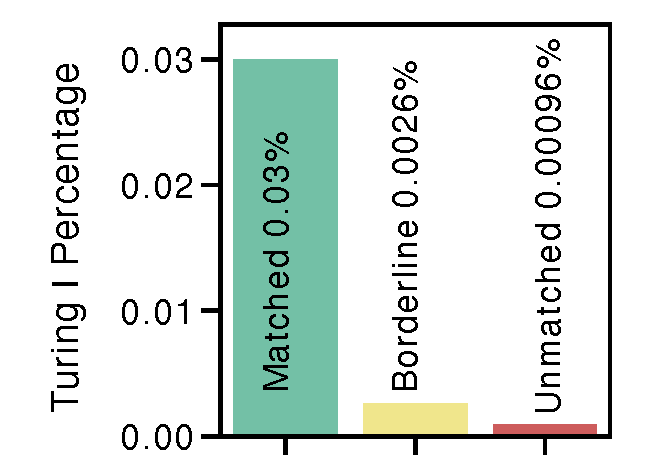
\includegraphics[width=0.6\textwidth]{chapters/Chapter 2/balancing_robustness}
    \caption{\textbf{Turing robustness as a percentage of parameter space with respect to matching of dose-response curves.} Turing instabilities include Turing I and Turing I-Hopf. Robustness from matched to unmatched increases 20-fold.}
    \label{fig:balancing_robustness}
\end{figure}

Following these insights, the transfer functions of the circuit components were matched experimentally by tuning the plasmid copy number,
the strength of ribosome binding sites (RBSs),
start codons and degradation tags~\parencite{Andersen1998, Wang2011,Hecht2017} by Dr.~Jure Tica and Tong Zhu.
Transfer function matching yielded a well-functioning circuit with a better capacity to produce spatial patterns
as discovered in this modelling study.
The matched dose-response curves can be seen in the next section in Fig.~\ref{fig:dose_response_experimental}.


\subsection{Parameter fine-tuning of the gene circuit to increase the likelihood of Turing patterns}
Another way of increasing the Turing parameter space is to tune parameters independently.
In this section, we explore the distribution of obtained Turing parameter sets
to understand how to tune each one to increase the robustness of our system.
Using the literature distribution defined above with only matched
parameter sets, we perform linear stability analysis to find Turing parameter sets.
In Fig.~\ref{fig:param_distributions_turing_vs_noturing},
we can observe how the distribution of Turing samples differs from the general sampling for each dimensionless parameter of the model.

\begin{figure}[H] % h! is a placement specifier; it tries to place the image here.
    \centering
    \begin{adjustbox}{center}
        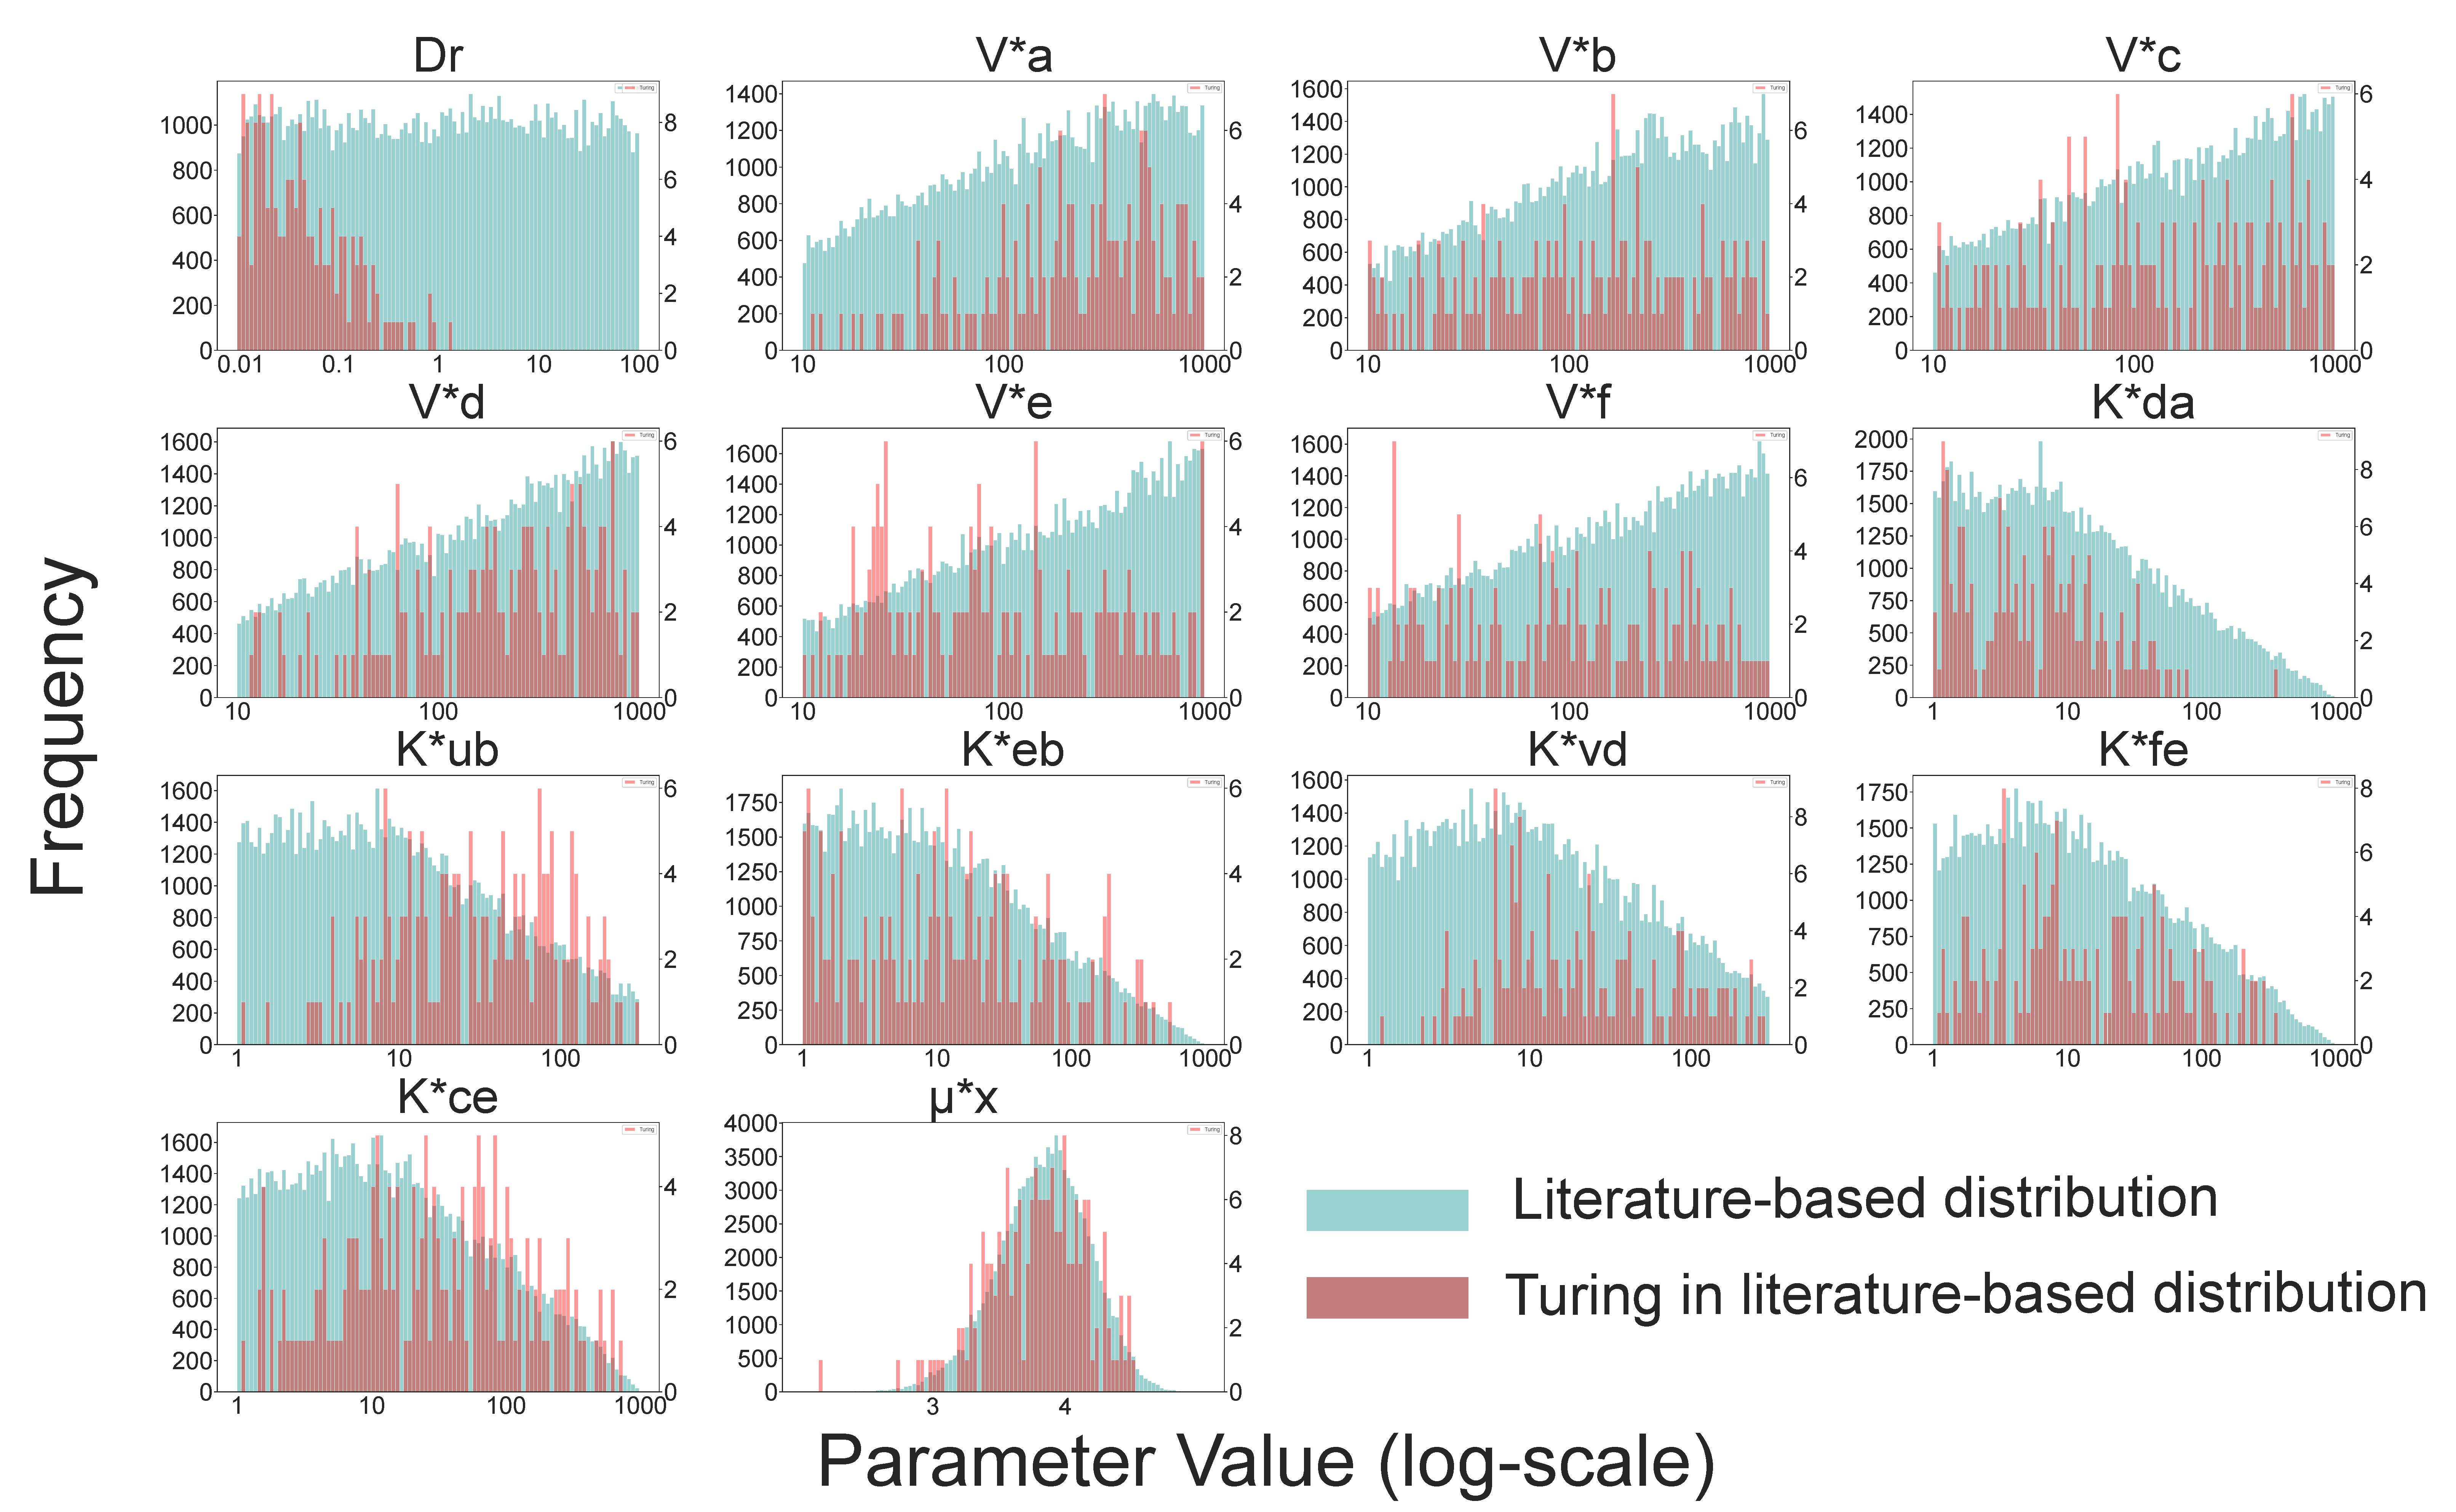
\includegraphics[width=1.2\textwidth]{chapters/Chapter 2/param_distributions} % The name of your image file; assumes it is in the same directory as your .tex file
    \end{adjustbox}
    \caption{\textbf{Broad literature-based distributions for model parameters} Distributions for dimensionless parameters of the model based on literature ranges.
    Blue distributions correspond to the sampled literature-informed distributions,
    where we made sure to only consider parameters where all the circuit transfer functions are matched.
    Red distributions correspond to Turing instabilities found in the blue distributions using linear stability analysis. Turing instabilities include Turing I and Turing I-Hopf. n's are ignored because they are fixed.}
    \label{fig:param_distributions_turing_vs_noturing} % A label for referencing this figure later in the document
\end{figure}

Turing pattern systems appear to have a bias for certain regions of parameters (Fig.~\ref{fig:param_distributions_turing_vs_noturing} red).
This is very clear for diffusion, where Turing patterns usually appear in regions with $D_r$ < 1.
$D_r$ is ($D_V / D_U$) meaning $OC_{14}$ should diffuse slower than pC.
Experimentally, the $D_{OC14}/D_{pC}$ ratio has been measured to show it is 0.25 (unpublished work,~\cite{tica_diffusers}).
This means our experimental setup has a diffusion ratio which is favourable for Turing pattern formation.
%where the DOC14/DpC ratio is approximately 0.25 in agar (1.4% w/V, 37 ºC) (Tica et al., unpublished observations).

Additionally, we used the model to study how to fine-tune the circuit using the exogenous tuning molecules IPTG, aTc and DAPG to increase Turing pattern likelihood.
$K_{da}^*$  and $K_{ce}^*$ are dependent on IPTG and aTC respectively, through an increasing function,
as seen in Eq.~\ref{kda_iptg} and Eq.~\ref{kce_atc}.
Therefore,
to understand the effects of these two exogenous tuning molecules we can look at their respective K parameters.
$K_{da}^*$ Turing parameters have a similar distribution to the sampled distribution,
implying that IPTG does not affect the robustness of the gene circuit to Turing pattern formation.
On the other hand, the $K_{ce}^*$ Turing parameters are more skewed to higher values than in the sampled distribution,
suggesting that aTc increases robustness for Turing pattern formation.
This is further shown by a more extensive sampling of the same distribution with five different $K_{ce}^*$ values
and measuring the Turing robustness in each
(Fig.~\ref{fig:atc_robustness})

\begin{figure}[H] % h! is a placement specifier; it tries to place the image here.
    \centering
    \begin{adjustbox}{center}
        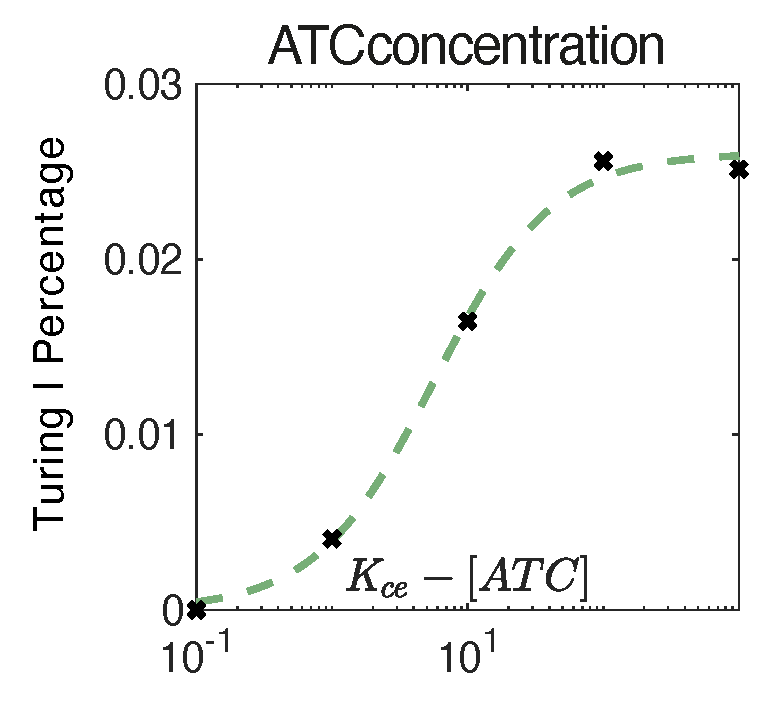
\includegraphics[width=0.5\textwidth]{chapters/Chapter 2/atc_robustness} % The name of your image file; assumes it is in the same directory as your .tex file
    \end{adjustbox}
    \caption{\textbf{Turing I robustness as a function of aTc or $K_{ce}$.} The highest Turing robustness is 0.025 with a high $K_{ce}$ value of $10^2$. After this, robustness plateaus or decays slightly. }
    \label{fig:atc_robustness} % A label for referencing this figure later in the document
\end{figure}

Finally, DAPG increases diffusor degradation by increasing $\mu_u$ and $\mu_v$,
however, these parameters are hidden in the dimensionless model,
where the diffusor equations were integrated into the protein equations.
As seen in Eqs~\ref{six_eq_dimensionless}b,d,f; $\mu_u$
and $\mu_v$ have a positively linear relationship with $K_{ub}^*$ and $K_{vd}^*$, respectively.
Both $K_{ub}^*$ and $K_{vd}^*$ have skewed distributions towards higher values compared to the sampled distribution
(Fig.~\ref{fig:param_distributions_turing_vs_noturing}).
This means that adding exogenous DAPG could also increase the robustness of the circuit for pattern formation.

In this section, we have obtained insights into parameter tuning
to understand how to optimise robustness for Turing pattern formation.
Following guidance from the model,
experimentalists went on to match the transfer functions of the circuit components and add high levels of aTc (10nM aTc).
Before testing the circuit for patterning,
experimentalists tested the behaviour of the circuit in liquid culture to make sure it behaved according to the design,
and that the transfer functions were matching.
Because the full circuit contains many closed-feedback loops, full-circuit liquid culture results are hard to interpret.
Hence,
subcircuit controls with no closed feedback loops were investigated
instead to test whether the circuit was well-matched and behaved as expected.
The conditions tested were under high aTc.
Some relevant subcircuits tested can be seen in Fig.~\ref{fig:dose_response_experimental} left.
The three subcircuits show how the dose-reponse curves are within the responsive ranges, as the green and red curves act according to the other (Fig.~\ref{fig:dose_response_experimental} right).
This means meaning the $K$ and $V$ parameters are within the matched region.
Subcircuit \#2 shows how the circuit is responsive to aTc which means aTc can be used for optimising Turing pattern robustness.

\begin{figure}[H] % h! is a placement specifier; it tries to place the image here.
    \centering
    \begin{adjustbox}{center}
        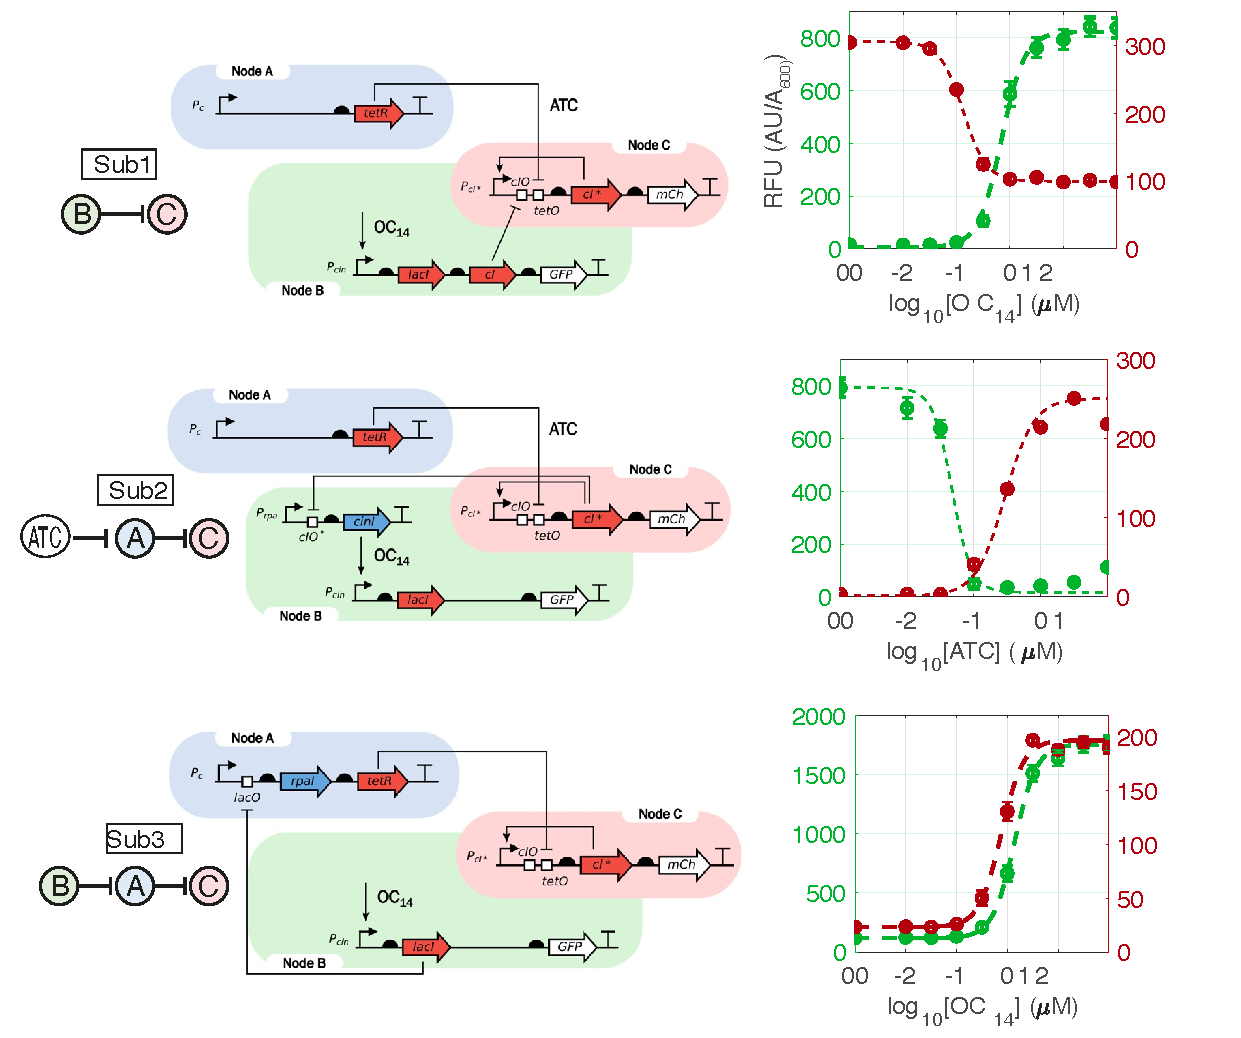
\includegraphics[width=1\textwidth]{chapters/Chapter 2/dose_response_experimental} % The name of your image file; assumes it is in the same directory as your .tex file
    \end{adjustbox}
    \caption{\textbf{Dose-response curves of subcircuits.}
    On the left, the three subcircuits Sub1, Sub2 and Sub3 are shown, which test interactions of the circuit. On the right, the dose-response curves correspond to each subcircuit produced by Dr.~Jure Tica and Dr.~Georg Wachter. Each curve shows liquid culture fluorescence in RFU units (y-axis) 18 hours after induction with different levels of inducer (x-axis).
    GFP on the left and mCherry on the right axis (unit AU/A600, mean ± SEM, n = 3). We can see all dose-response curves are matched as in Sub1 and Sub3, red responds to the green and in Sub2 green responds to the red. Sub1 and Sub3 were tested under 10nM aTc.}
    \label{fig:dose_response_experimental} % A label for referencing this figure later in the document
\end{figure}
\section{Constrained parametrised distributions:
fitting to liquid culture data of gene subcircuits}\label{Constrained parametrised distributions: fitting to liquid culture data of gene subcircuits}
The dose-response curves obtained (Fig.~\ref{fig:dose_response_experimental} left)
are not only useful to characterise the circuit,
but also for the parametrisation of the model.
Using the dimensionless model,
the fluorescence dose-response curves \#1 and \#3 can be fitted
to obtain values for $K_{XY}$ and $V_{X}$ using a multivariate analysis approach.
This is possible because the non-dimensionalisation facilitates the comparison between the model and experimental dose-response curves with simple and intuitive methods.


\subsection{Steady-state subcircuit equations for fitting.}
As previously seen in Eq.\ref{1toVmax},
the non-dimensionalisation transforms the dose-response range so it goes from 1 to $V_{X}+1$.
This transformation can be seen in Fig.~\ref{fig:dose_response_transforms}, right.
For the experimental data to match the model,
it is divided by the smallest fluorescence value within each experiment and is expressed in relative fold-change units
(Fig.~\ref{fig:dose_response_transforms}, left).
Fold-change units can take values from 1 to $F_{\max}/F_{\min}$
(maximal and minimal fluorescence levels in the original, untransformed dataset, respectively).
Because the dose-response curves of subcircuit \#1 and subcircuit \#3 are OC14-dependent, the experimental OC14 units (µM) are also non-dimensionalised using the transform
\begin{equation}
    [B*]=[OC_{14}] \cdot \frac{\mu_{b}\mu_{v}}{k_{2}b_{B}}
    \label{Btransform}
\end{equation}
Now the dimensionless model dose-response curves and experimental dose-response curves are both expressed on relative scales and are compatible for fitting (Fig.~\ref{fig:dose_response_transforms}, bottom).
\begin{figure}[H] % h! is a placement specifier; it tries to place the image here.
    \centering
    \begin{adjustbox}{center}
        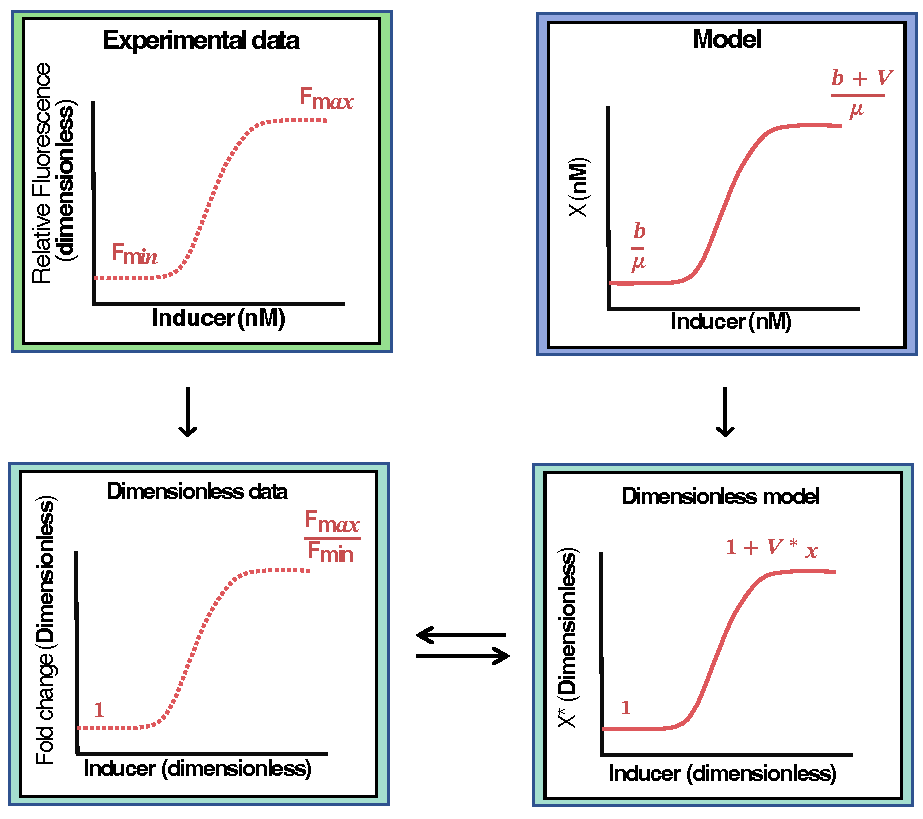
\includegraphics[width=0.8\textwidth]{chapters/Chapter 2/dose_response_transforms}
    \end{adjustbox}
    \caption{\textbf{Experimental data and model transformation for parametrisation.} Experimental data is scaled by the smallest fluorescence value, so the minimum value is 1 (left). The model is nondimensionalised
    as explained in the sections above so the smallest value is 1
    and biggest is $V_{X} +1$ (right).
    In both cases, units are dimensionless, and the basal level is 1 (bottom).}
    \label{fig:dose_response_transforms}
\end{figure}


The models for the subcircuits are derived from the main PDE system (Eqs.~\ref{six_eq_dimensionless}).
Subcircuit \#1 only involves species [F] and [E] (cI and cI*), whereas subcircuit \#3 involves species [C], [D] and [E]
(TetR, LacI and cI*).
Detailed diagrams of these two subcircuits can be found in Fig.~\ref{fig:dose_response_experimental} left.
All other species are set to zero.
For the model parametrisation, based on the subcircuit designs,
we derive steady-state expressions for the dynamically regulated species so that
\begin{equation}
    \pdv{X}{t}=0; \quad X=X_{eq}
\end{equation}

For Subcircuit \#1 we obtain the following steady-state expressions:

\begin{subequations}\label{Subcircuit 1 equations}
\begin{equation}
    F_1 = 1 + V_f \left( \frac{1}{1+ \left( \frac{\mu_v K_{vd}}{k_v [O_{C14}]} \right)^{n_{vd}}} \right)
\end{equation}
%\begin{equation}
%    E_1 = 1 + V_e \left( 1+ \left( \frac{1 + V_f \left( \frac{1}{1+ \left( \frac{\mu_v K_{vd}}{k_v [O_{C14}]} \right)^{n_{vd}}} \right)}{K_{fe}} \right)^{n_{fe}} \right)^{-1}
%\end{equation}
\begin{equation}
    E_1 = 1 + V_e \left( \frac{1}{1+ \left( \frac{F_1}{K_{fe}} \right)^{n_{fe}}} \right)
\end{equation}
\end{subequations}

For Subcircuit \#3 we obtain the following steady-state expressions:
\begin{subequations}\label{Subcircuit 3 equations}
\begin{equation}
    D_3 = 1 + V_d \left( \frac{1}{1+ \left( \frac{\mu_v K_{vd}}{k_v [O_{C14}]} \right)^{n_{vd}}} \right)
\end{equation}
\begin{equation}
    C_3 = 1 + V_c \left( \frac{1}{1+ \left( \frac{D_3}{K_{da}} \right)^{n_{da}}} \right)
\end{equation}
\begin{equation}
    E_3 = 1 + V_e \left( \frac{1}{1+ \left( \frac{C_3}{K_{ce}} \right)^{n_{ce}}} \right)
\end{equation}
\end{subequations}

\subsection{Fitting process and the resulting best-fit distributions.} \label{Fitting process and the resulting best fit distributions.}
In addition to scaling and nondimensionalising, the lowest GFP data points were excluded,
because fluorescence readings were insufficiently sensitive
to measure concentration at these points (Fig.~\ref{fig:dose_response_experimental}).
This improved the quality of the fit and allowed us to identify a broader range of suitable solutions.

The two-equation systems Eqs.~\ref{Subcircuit 1 equations},\ref{Subcircuit 3 equations}
are fitted independently to the experimental dataset with the python \textit{scipy.optimize.curve\_fit} package,
which uses the Levenberg-Marquardt to minimise the sum of squared errors (SSE), given by
\begin{equation}
    SSE = \sum_{i=1}^{i} (y_{i}-f(x_{i}))^2
\end{equation}

where $y_i$ is the experimental data
and $f(x_i)$ are the two systems of equations
parameterised by $V^*_{C}$, $V^*_{D}$, $V^*_{E1}$, $V^*_{E3}$, $V^*_{F}$, $K^*_{vd}$, $V^*_{fe}$, $V^*_{da}$
and $V^*_{ce}$.
The minimisation algorithm generates a vector of best-fit parameters $k$

\begin{table}[H]
    \centering
    \begin{tabular}{|c|c|c|c|c|c|c|c|c|}
        \hline
        \textbf{$V^*_{C}$} & \textbf{$V^*_{D}$} & \textbf{$V^*_{E1}$} & \textbf{$V^*_{E3}$} & \textbf{$V^*_{F}$} & \textbf{$K^*_{vd}$} & \textbf{$V^*_{fe}$} & \textbf{$V^*_{da}$} & \textbf{$V^*_{ce}$} \\
        \hline
        9.95 & 6.50 & 1.99 & 7.8 & 3.64 & 18.94 & 2.26 & 67.92 & 3.47 \\
        \hline
    \end{tabular}
    \caption{\textbf{Vector of best fit parameters $k$}}
    \label{table:bestfit table}
\end{table}


Two best-fit parameters are obtained for $V^*_{E}$ as this parameter is present in both subcircuit models.
However, only $V^*_{E1}$ from subcircuit \#1 is considered.
These parameters are used to generate the following dose-response curves (Fig.~\ref{fig:dose_responses_bestfit}).


\begin{figure}[H] % h! is a placement specifier; it tries to place the image here.
    \centering
    \begin{adjustbox}{center}
        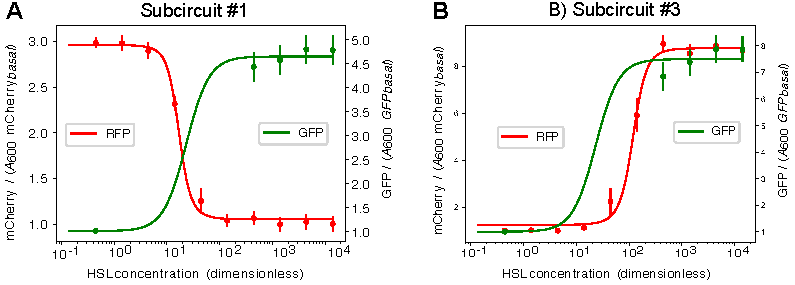
\includegraphics[width=1\textwidth]{chapters/Chapter 2/dose_responses_bestfit} % The name of your image file; assumes it is in the same directory as your .tex file
    \end{adjustbox}
    \caption{\textbf{Best fit for processed data set.} Processed dataset is fitted using \textbf{(A)} Eq.~\ref{Subcircuit 1 equations} for subcircuit \#1 and \textbf{(B)} Eq.~\ref{Subcircuit 3 equations} for subcircuit \#3.}

    \label{fig:dose_responses_bestfit} % A label for referencing this figure later in the document
\end{figure}


The minimisation algorithm produces a covariance matrix $C_k$. This covariance matrix can also be understoood as the inverse of the Hessian matrix which represents the derivative of the loss function in the different parameter dimensions.
In other words, this Hessian matrix represents how the loss increases or decreases when parameters are varied together

\begin{equation}
    H_{L_{k}} = \begin{bmatrix}
                     \frac{\partial^2 L}{\partial k_1^2} & \frac{\partial^2 L}{\partial k_1 k_2} & \cdots & \frac{\partial^2 L}{\partial k_1 k_{n}} \\
                     \frac{\partial^2 L}{\partial k_2 k_1} & \frac{\partial^2 L}{\partial k_2^2} & \cdots & \frac{\partial^2 L}{\partial k_2  k_{n}} \\
                     \vdots & \vdots & \ddots & \vdots \\
                     \frac{\partial^2 L}{\partial k_{n}k_1} & \frac{\partial^2 L}{\partial k_{n}  k_2} & \cdots & \frac{\partial^2 L}{\partial k_{n}^2}
    \end{bmatrix}
\end{equation}


A multivariate Gaussian distribution is generated using $k$ and $C_{k}$
\begin{equation}
    X \approx N(k,C_k)
\end{equation}

with a probability density function $p(x;k,C_k )$

\begin{equation}
    p(x;k,C_k )= \frac{\exp\left(-\frac{1}{2} (x - k)^\top C_k^{-1} (x - k)\right)}{\sqrt{(2\pi)^k C_k}}
\end{equation}

The multivariate Gaussian distribution is the generalization of a normal distribution to higher dimensions.
For example, for 2-dimensional Gaussian distributions,
when the covariance of two parameters X and Y is positive, the parameters are positively correlated
(Fig.~\ref{fig:multivariate_gaussians}, right).
This means that if the parameters are increased together, the behaviour of the system should change minimally
(and the error to the data should not increase).
On the other hand, a negative covariance leads to an inverse correlation of the parameters,
meaning when one increases the other should decrease to ensure the error does not increase
(Fig.~\ref{fig:multivariate_gaussians}, left).
Finally, a covariance of zero means the X and Y parameters are completely independent,
producing a circular distribution (Fig.~\ref{fig:multivariate_gaussians}, center).

\begin{figure}[H] % h! is a placement specifier; it tries to place the image here.
    \centering
    \begin{adjustbox}{center}
        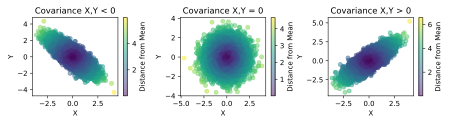
\includegraphics[width=1\textwidth]{chapters/Chapter 2/multivariate_gaussians} % The name of your image file; assumes it is in the same directory as your .tex file
    \end{adjustbox}
    \caption{\textbf{Multivariate Gaussian distributions.} Pairplots of X and Y parameter distributions with (left) negative covariance, (centre) zero covariance and (right) positive covariance.
    The colour represents the distance to the mean, or in other words to the best-fit parameter ($k$).
    Blue are the parameter ($k$) with minimal loss and yellow are neighbouring parameters with bigger loss.}
    \label{fig:multivariate_gaussians} % A label for referencing this figure later in the document
\end{figure}

The multivariate Gaussian distribution generated from the vector of best-fit parameters $k$ and the covariance matrix $C_{k}$ can be seen as a pairplot in Fig.~\ref{fig:multivariate_from_fit}.
Positive, negative and no correlations were observed in these distributions.
This figure shows how certain parameters have positive covariance such as $V^*_c$ and $K^*_{ce}$.
A high $V^*_c$ indicates a strong production of TetR, while a high $K^*_{ce}$ indicates a higher concentration of TetR to have the same inhibition effects.
Therefore, if both are increased together, the behaviour of the system should remain the same and the dose-response fit should be unaltered.
Some parameters have a negative covariance such as $K^*_{vd}$ and $K^*_{fe}$.
While a high $K^*_{vd}$ decreases the production of cI, a low $K^*_{fe}$ decreases the amount of cI needed to have the same inhibition effects.
Therefore if varied in opposite directions, the circuit behaviour remains unaltered.
Others are independent like $V^*_{d}$ and $K^*_{f}$ which determine the production rates of the molecules LacI and cI which affect the circuit independently.

\begin{figure}[H] % h! is a placement specifier; it tries to place the image here.
    \centering
    \begin{adjustbox}{center}
        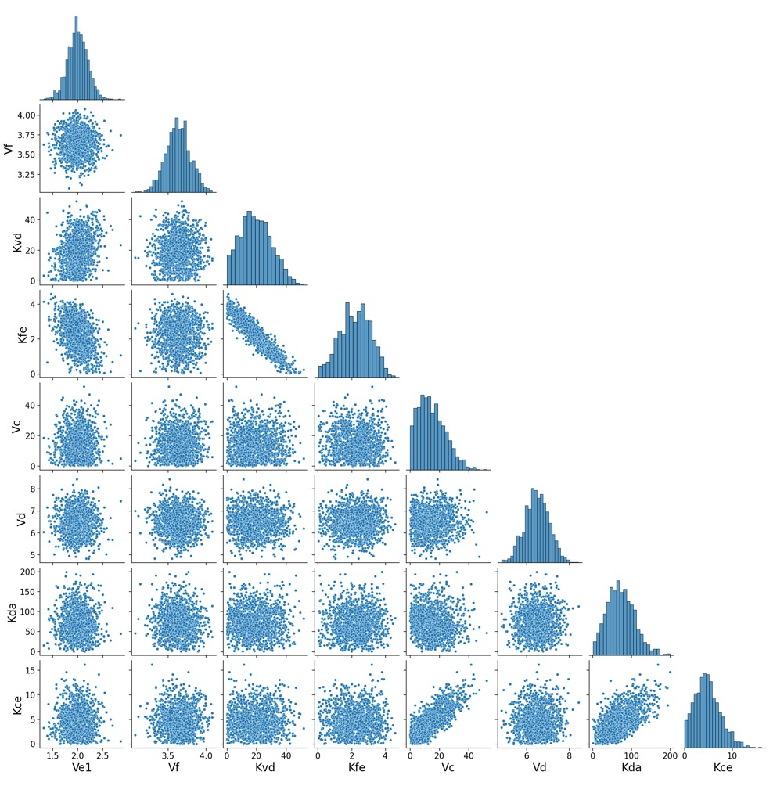
\includegraphics[width=1\textwidth]{chapters/Chapter 2/multivariate_from_fit} % The name of your image file; assumes it is in the same directory as your .tex file
    \end{adjustbox}
    \caption{\textbf{Multivariate Gaussian distributions for fitted parameters.}
    Pairplot of distribution resulting from fitting subcircuit \#1 and \#3, using $q=10$.
    This distribution has a probability density function $p(x;k,10\cdot C_{k})$
        where $k$ is the best fit parameter vector and $C_{k}$ is the covariance matrix.
    Diagonals represent the univariate distributions.
    The non-diagonals represent the multivariate distributions of parameter pairs, where we can observe positive and negative correlations as well as independent pairs of parameters. Negative parameters are removed from the distribution as these are biologically not possible.}
    \label{fig:multivariate_from_fit} % A label for referencing this figure later in the document
\end{figure}

The width of the multivariate Gaussian distributions can be increased by multiplying $C_k$ by a scalar factor $q$ where $q>1$.
This process unconstrains the fits and allows more error with respect to the experimental data.
To search for Turing patterns close to the fitted parameter combination $k$,
the value of $q$ is progressively increased until a Turing parameter set is found through linear stability analysis.
Through this process, the first 3 Turing parameter combinations are found with $q=10$.
These are the closest Turing solutions to the best fit parameter combinations.
The dose-response curves
generated by the $q=10$ distribution are shown in Fig.~\ref{fig:dose_response_multivariate_gaussian}.
Within all the curves shown, 3 of them are generated by Turing parameter sets.
The three Turing parameter sets are ensured to be ‘balanced’,
where the input/output relationships of the components are matched (see Section~\ref{balancing}).

\begin{figure}[H] % h! is a placement specifier; it tries to place the image here.
    \centering
        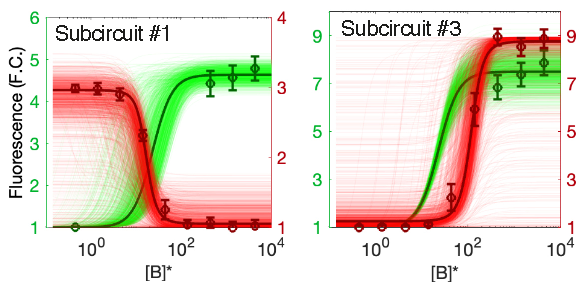
\includegraphics[width=1\textwidth]{chapters/Chapter 2/dose_response_multivariate_gaussian} % The name of your image file; assumes it is in the same directory as your .tex file
    \caption{\textbf{Fitted OC14 dose-response curves
    produced using the multivariate Gaussian distributions.}
    Dots show experimental data,
        the thick line is generated from best fit parameters and the thin lines are derived from multivariate Gaussian distributions cantered around the best fit with $q=10$.
        The parameters used to generate these curves come from the multivariate analysis optimisation, for subcircuit 1 (left) and subcircuit 3 (right). The parameter distributions are shown in Fig.~\ref{fig:multivariate_from_fit}}
    \label{fig:dose_response_multivariate_gaussian} % A label for referencing this figure later in the document
\end{figure}
The corresponding $q=10$ multivariate Gaussian parameter distributions are shown in Fig.~\ref{fig:multivariate_from_fit}.
The distributions of the multivariate Gaussian in 1-parameter dimension and the Turing parameter sets are shown in Fig.~\ref{fig:1d_distributions}.
This figure shows where the parameters of Turing solutions lie in comparison with the fitted distributions.
Overall, only parameter $K^*_{da}$ is far off from the Turing solutions.
Lower values of $K^*_{da}$ would be required to increase the likelihood of finding Turing solutions.
This K*da parameter, which is captured in Subcircuit \#3 (see Eq.~\ref{Subcircuit 3 equations}b), has the highest uncertainty because nodeA is hideden and we therefore need to infer two functions with one curve.
%TODO add starts to params

\begin{figure}[H] % h! is a placement specifier; it tries to place the image here.
    \centering
    \begin{adjustbox}{center}
        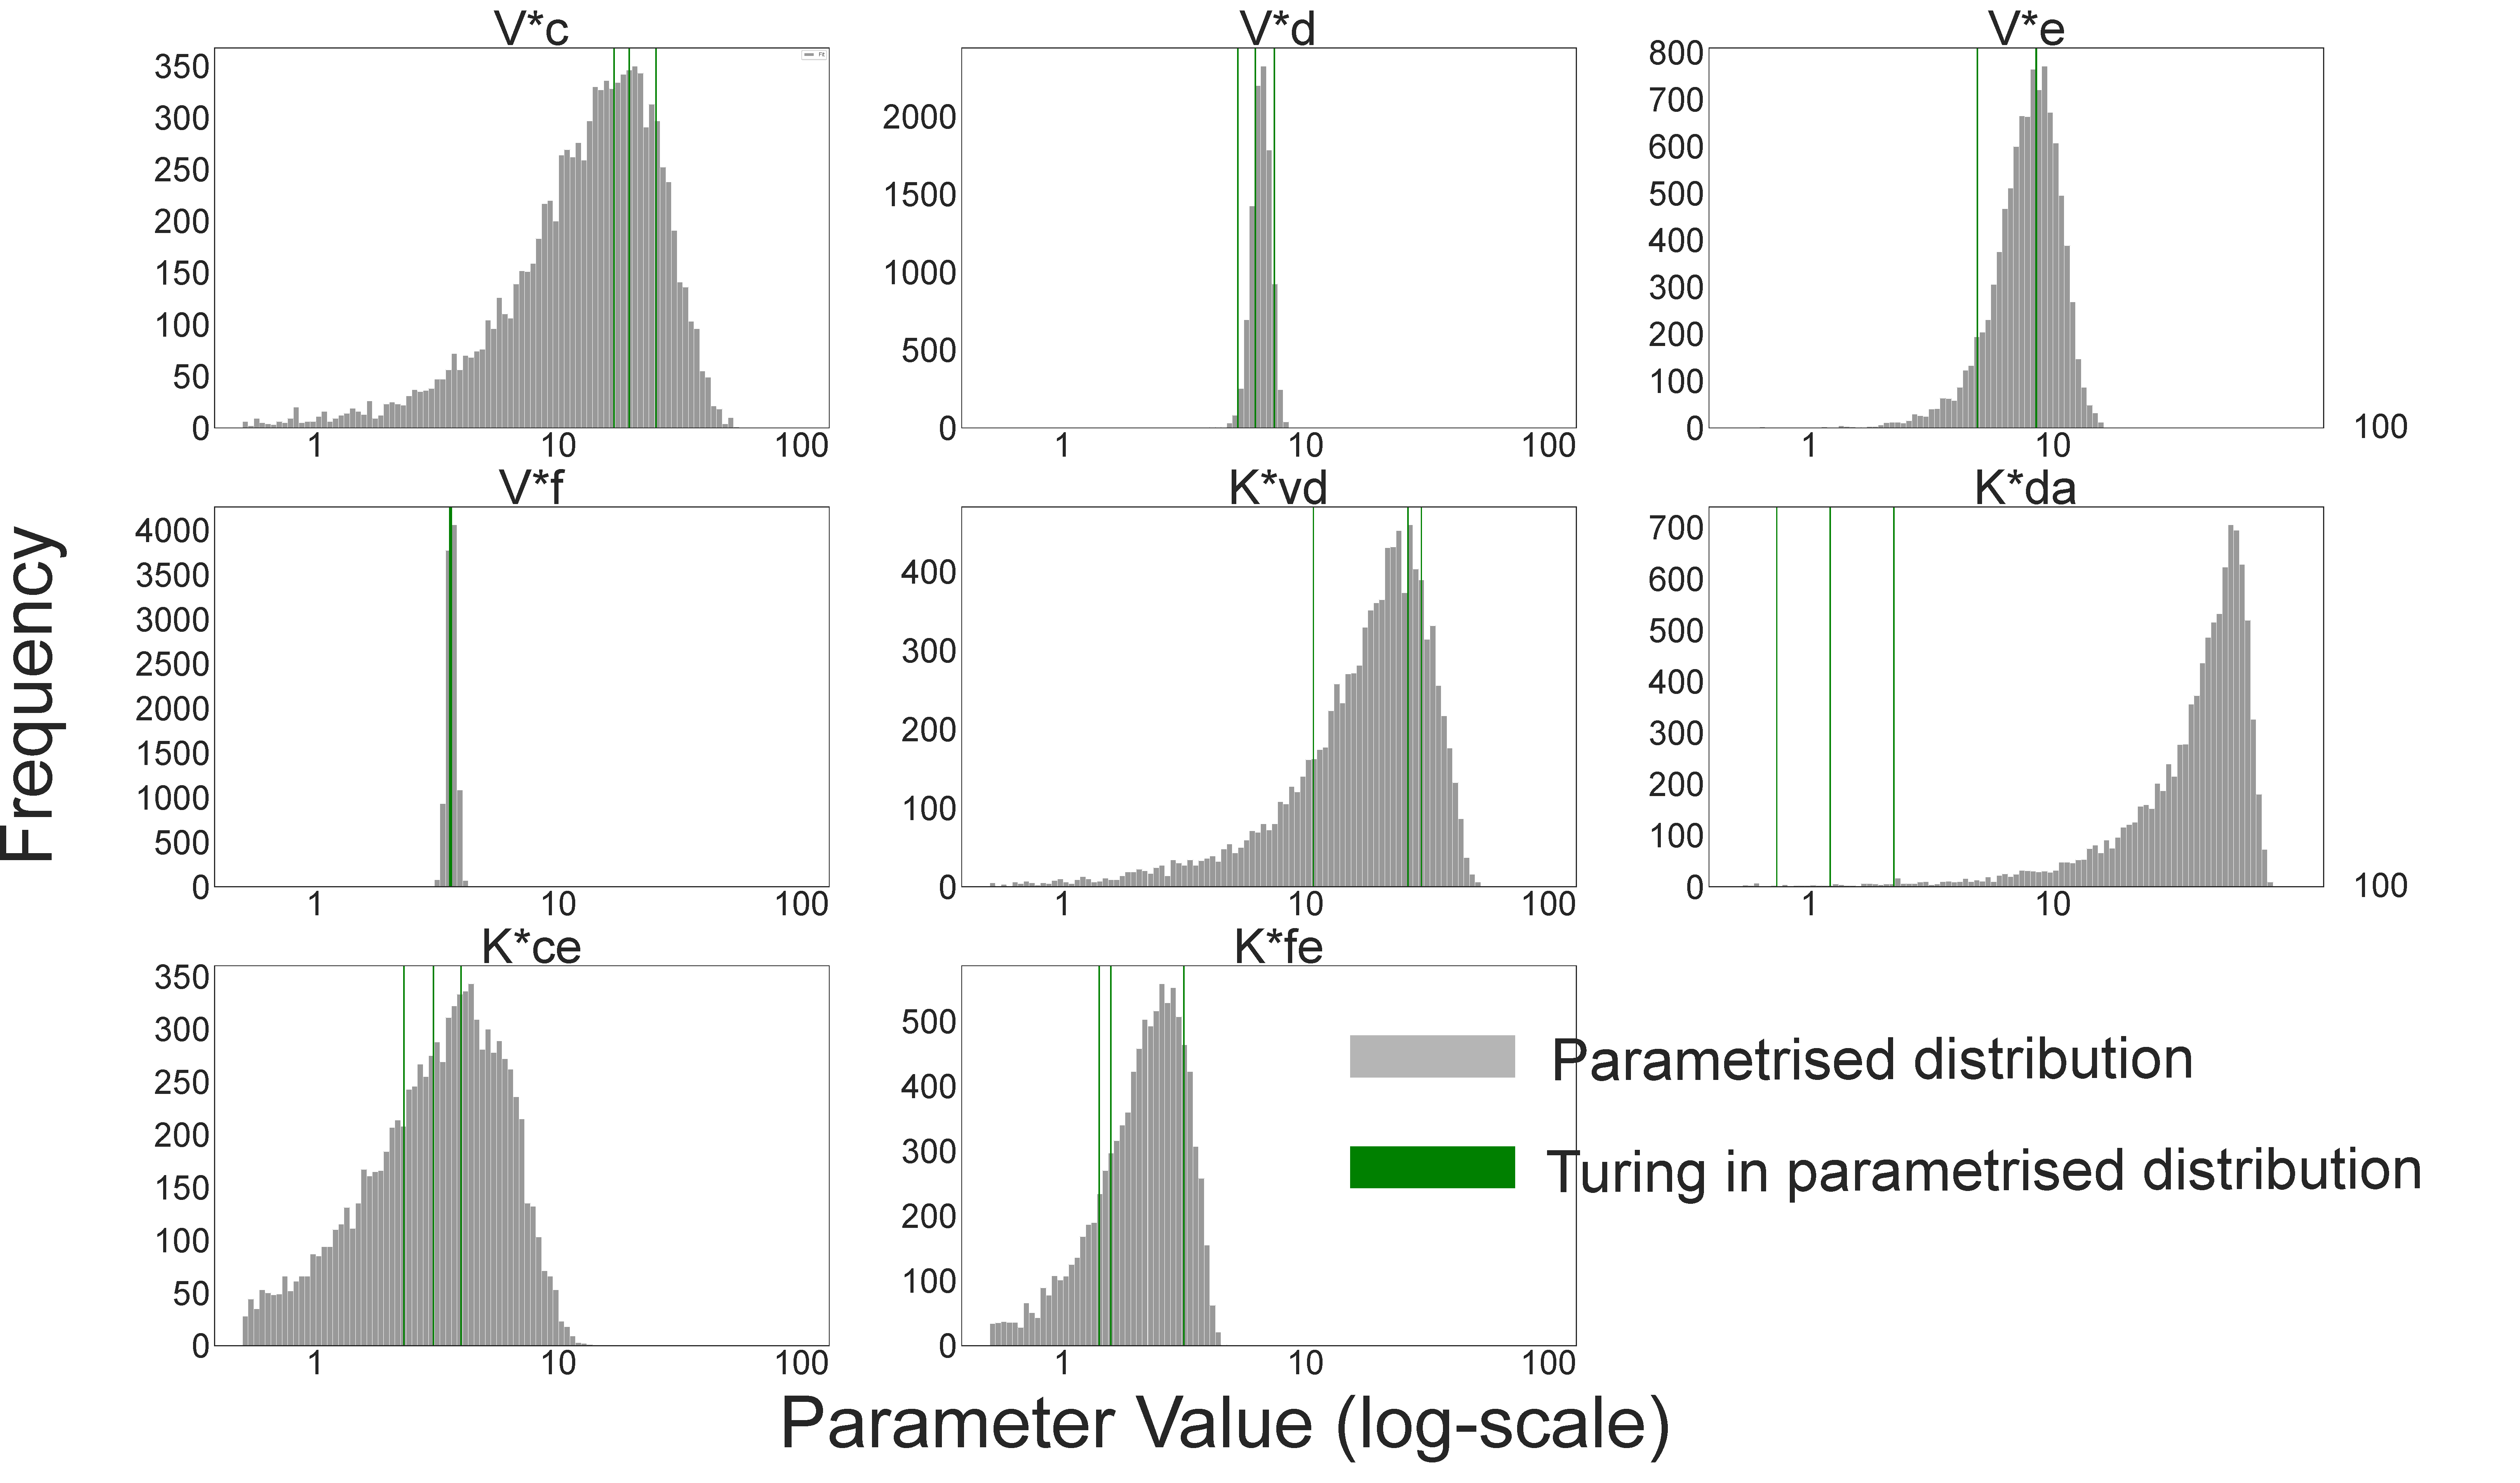
\includegraphics[width=1\textwidth]{chapters/Chapter 2/1d_distributions} % The name of your image file; assumes it is in the same directory as your .tex file
    \end{adjustbox}
    \caption{\textbf{Constrained parametrised distributions for $V^*_X$ and $K^*_{XY}$ parameters in 1 dimension.}
    Distributions for dimensionless parameters based on fitting to liquid-culture experimental data.
    Grey distribution corresponds to parameters from fitting with $q=10$.
    Green vertical lines correspond to the 3 Turing parameter sets
    found in the grey distribution using linear stability analysis. Parameters which generate non-matched dose-response curves are removed.}
    \label{fig:1d_distributions} % A label for referencing this figure later in the document
\end{figure}

\section{Discussion}
A synthetic gene circuit was built with the aim of engineering periodic pattern formation in synthetic \textit{E.~coli} biofilms (Fig.~\ref{fig:synthetic circuit_chapter2}).
This chapter described the model built to understand the spatio-temporal dynamics of this synthetic gene circuit.
The parameter space was explored to show the circuit can produce Turing patterns, and in certain regions, the likelihood of finding these patterns is higher.
Finally, the model was parametrised using liquid culture data to constrain the model parameters to experimentally realistic values.

\subsection{Model of synthetic gene circuit \#1754}
The model presented was a PDE system which describes the concentrations of the six proteins in space and time.
This model gives us insights into how protein concentrations change over time and in space and whether any spatio-temporal patterns form.
Because the experimental circuit is the largest \acrfull{RD} gene circuit ever built, the model is highly complex with many variables and parameters.
This results in computationally expensive numerical simulations and a high-dimensional parameter space with over 20 dimensions, which is complicated to sample.

To simplify the model, many assumptions were made.
For example, quasi-steady states were assumed for mRNA production, protein-promoter binding, receptor-diffusor binding and diffusor synthesis.
Although these processes exist in a quasi-steady state equilibrium, they might produce delays which are not taken into account in this model.
Investigating these delays would be necessary in the future to understand whether they disrupt pattern formation as shown in~\cite{Maini2012}.
Additionally, degradation was assumed to be linear, which might not be accurate in some cases.
High levels of proteins, burden or age-dependent effects might collapse the degradation machinery~\parencite{kintaka2020genetic} leading to non-linear dynamics which are not currently captured.
Additionally, diffusor precursors as well as diffusor receptors were assumed to be in excess to avoid extra equations and parameters.
The parameters of the model were also assumed to be constant over time, which might not be realistic due to cell burden, nutrient depletion or other effects in the biofilm.
Future work in this direction would involve exploring experimentally the relationship between these effects and the model parameters.
An interesting example of this would be to define a time-dependent nutrient equation on which kinetic parameters are dependent.
Finally, this model assumed fluorescent protein concentration is linearly correlated with fluorescence.
Although this assumption is often correct~\parencite{soboleski2005green, csibra2022absolute}, several factors can disrupt the linearity.
For example, low concentrations of fluorescent protein might not be detected by the instruments, leading to a non-linear relationship.
pH and temperature can also affect fluorescent values~\parencite{ward1982spectral}.
When using LacI and cI* to model GFP and RFP fluorescence respectively, we need to take into account these assumptions on linearity and understand when they might break.

\subsection{Finding Turing instabilities and optimising Turing robustness}
Regardless of all the assumptions, the model was extremely useful in giving us insights into the system.
Firstly, the model parameter space was searched using linear stability analysis to find Turing I instabilities.
Turing I-Hopf instabilities were also searched for, as they have been shown to produce stationary periodic patterns in many cases as seen in Section~\ref{nogrowth}.
The model did produce Turing I and Turing I-Hopf instabilities, meaning periodic stationary patterns as the ones observed in Fig.~\ref{fig:square_turing} could occur experimentally.
When the gene circuit was built inspired by the original \#1754 topology,
more nodes and connections had to be implemented to replicate the original functions.
Therefore, it was unclear whether these changes would remove the capabilities of patterning.
Proving the genetic implementation of this topology could produce patterning was necessary before searching for Turing patterns experimentally.

The model also helped understand parameter regimes in which the gene circuit was more likely to produce Turing instabilities, including both Turing and Turing I-Hopf.
By matching circuit components to have responsive dose-response curves, the robustness could be increased 20-fold from 0.001\% to 0.19\% as seen in Fig.~\ref{fig:balancing_robustness}.
This robustness could be further increased by tuning specific parameters such as decreasing the $D_{OC14}/D_{pC}$ ratio, increasing aTc or increasing DAPG.
Different levels of aTc were explored in a system with matched dose-response curves.
It was seen that robustness could be increased from 0 to 0.025 by increasing $K_{ce}$, which is equivalent to adding exogenous aTc to the experiment.

These results guided the experimental fine-tuning of the circuit by matching dose-response curves and adding exogenous aTc and DAPG.
Decreasing $D_{r}$ is harder, as there is no current good method for controlling the diffusion of quorum sensing molecules.
A potential route of decreasing the diffusion rate of a quorum-sensing molecule is through receptor sequestering:
When the number of receptors is much larger than the number of quorum sensing ligands,
there is an irreversible uptake of some molecules which has been linked to shorter range communication (i.e. slower diffusion constants~\parencite{vangestel}).
Therefore, to decrease $D{r}$,
we can slow down the diffusion of $OC_{14}$ by increasing the expression of the CinR receptor which will bind to $OC_{14}$.
This can be done by tuning the RBS for higher expression.

Overall, this model enabled us to design experimental strategies for tuning the robustness of the system so Turing patterns could be obtained experimentally.
However, it is important to note that although they have been optimised, the robustness levels obtained are still extremely low.
Further investigation to understand how to further increase the percentage of Turing solutions in parameter space is needed.
In this thesis, robustness optimisation was carried out by tuning model parameters.
However, it is worth investigating whether growth, boundary conditions or even a pre-pattern could increase the probability of obtaining Turing patterns with this circuit.

\subsection{Model parametrisation}
Working with large parameter spaces based on literature parameters is useful for understanding the overall potential of the circuit architecture.
However, once the system is fine-tuned by matching dose-response curves and adding exogenous aTc, it is important to constrain the parameter space to that of the fine-tuned circuit, so more accurate results are produced.
Additionally, because of the high dimensionality of the parameter space, it is useful to parametrise the model to obtain a smaller parameter space which is easier to sample.
Dose-response curves from the fine-tuned circuit in liquid culture were produced which could be used for parametrisation.
Parametrisation was possible because of the dimensionless model.
This dimensionless model could produce dose-response curves such as the experimental ones by taking the steady state expressions under different inducer concentrations (Eqs~\ref{Subcircuit 1 equations},~\ref{Subcircuit 3 equations}).
Relative fluorescent units from the experimental dose-response curves could be directly compared to dimensionless units of our dimensionless model as seen in Fig.~\ref{fig:dose_response_transforms}.

It is important to note that the experimental data used for parametrisation represents the behaviour of cells in liquid culture.
Parameters might vary slightly for cells growing in colonies on agar surfaces, especially as they become old.
Dose-response curves in agar could be produced in the future.
This would allow us not only to understand the parameters of cells growing in agar dishes, but also have different fits for old cells in the middle and new cells at the edge of the colony.

By fitting the dose-response models to the experimental liquid culture data, we aimed to obtain a distribution of model parameters that replicated the experimental data with a certain level of uncertainty.
A distribution is preferred over a single fit as biological systems exhibit noise and there is a certain level of uncertainty in the fixed parameters of the model.
This distribution could be obtained by using a Bayesian approach or a multivariate Gaussian optimisation approach.
With Approximate Bayesian Computation, a prior is given which is updated by sampling the parameter space to obtain a posterior distribution that fits the data.
This Bayesian approach works well if prior knowledge needs to be incorporated into the model and if non-linear relationships between parameters are present.
However, it is more computationally expensive.
On the other hand, multivariate Gaussian optimisation is a much more computationally efficient algorithm based on a simple least squares minimisation to produce a mean value and a covariance matrix.
This algorithm is less flexible in terms of the prior given and the relationships between parameters (i.e.~non-linearities are not captured).
Additionally, the distribution is only centred around the best fit mean value, meaning the posterior might be limited.

Using the multivariate Gaussian approach, a distribution of parameters was obtained
which fitted the experimental dose-response with a certain level of uncertainty.
This allowed for a much more constrained parameter space which is easier to sample and gives more accurate results.
Additionally, the fitting process allowed us to understand and verify correlations between parameters.
All these correlations can be explained using the logic of the circuit architecture, which means the distributions are correct and the model accurately describes the dynamical behaviour of the circuit.
Interestingly, Turing solutions were found within these distributions.
Theoretically, these Turing solutions are the closest solutions in parameter space that fit the experimental data.
Therefore, we should expect their dynamic behaviour to match the experiments more closely than any other Turing solution found in the literature-based parameter space.

However, a high level of uncertainty ($q=10$) was needed to find such Turing solutions in the distribution.
This lack of robustness in the fitted distribution can be attributed mainly to the $K^*_{da}$ parameter, which has a higher distribution than Turing solutions.
This $K^*_{da}$, which is the $[LacI]$ needed for half repression of node A, is an uncertain parameter as no fluorescent reporters are linked to node A.
Currently, the only data used is on node B, with a GFP reporter, and node
C, with an mCherry reporter.
Having dose-response curves which report on every gene of the circuit would get rid of issues on node A parametrisation, and potentially increase the Turing robustness in the fitted distribution.
A potential route to improve this parametrisation technique would be to use RT-qPCR, which is a technique used for mRNA quantification.
mRNA counts of every one of the six genes would be measured for different inducer concentrations, hence obtaining information on the currently 'hidden' nodes.
Additionally, because fluorescence levels are sometimes not an accurate predictor of protein levels as previously discussed, using mRNA counts would improve issues such as the low fluorescent values not being detected.
Overall, this parametrisation method goes beyond studying pattern formation and could be useful to parametrise any genetic circuit model in synthetic biology.


As we reflect on the work presented in this chapter, the significance of optimizing Turing pattern robustness through precise parameter tuning becomes clear.
Additionally, our parametrization approach and the subsequent uncovering of Turing patterns present within experimentally relevant parameter distributions stand as a testament to the power of using mathematical models in synthetic biology.
The insights gleaned from this study illuminate the path forward not only for the engineering of synthetic \textit{E. coli} biofilms, which is done in the next chapter, but also for the broader engineering of genetic circuits in complex biological systems.
As we continue to fine-tune these parameters, our ability to predict and control the dynamical behavior of synthetic gene circuits will advance, leading to more robust and reliable applications in biotechnology.
